\chapter{粲介子半轻单举衰变的理论研究}
本章从幂次修正和微扰修正两方面介绍本研究的相关工作：对于幂次修正，本文详细讨论了树图水平上量纲三与量纲五算符对应Wilson系数的匹配与相空间解析积分。对于微扰修正，本文讨论了单圈水平上领先幂次修正的解析积分，并给出电子能谱的解析形式。此外简单介绍了高量纲算符的参数化方案。
\section{幂次修正}
\subsection{B介子半轻单举衰变}
本节以$\mrm{b \to c}$和$\mrm{b \to u}$过程为例，讨论树图水平上量纲三与量纲五算符对应Wilson系数匹配和相空间解积分，可得$\mrm{b\to c}$和$\mrm{b\to u}$衰变过程的电子能谱和衰变宽度。

$\mrm{b \rightarrow c \ell \nu}$过程的弱有效哈密顿为\ct{manohar2000heavy}
\begin{equation}
    \mathcal{H}_W=\frac{4 \mrm{G_F}}{\sqrt{2}} \mrm{V}_{\mathrm{CKM}}\left(\bar{q} \gamma_\mrm{L}^\mu\mrm{c}\right)\left(\bar{\nu}_{\ell} \gamma_{\mrm{L} \mu} \ell\right)=\mrm{\frac{4 G_F}{\sqrt{2}} V_{\mathrm{CKM}} }J_\mrm{q}^\mu J_{\mrm{\ell} \mu},
    \end{equation}
其中, $\gamma_\mrm{L}^\mu=\gamma^\mu P_\mrm{L}, P_\mrm{L}=\left(1-\gamma_5\right) / 2$ 是左手投影算符, $\mrm{G_F}$ 是费米常数, $\mrm{V}_{\mathrm{CKM}}$是相关的Cabibbo-Kobayashi-Maskawa（CKM）矩阵元模方, $J_\mrm{q}^\mu$ and $J_{\mrm{\ell}}^\mu$ 分别是强子和轻子流。基于洛伦兹对称性和宇称-电荷共轭对称性，强子流对应振幅模方\footnote{轻子流对应振幅模方是$ L^{\alpha \beta}=2\left(p_\mrm{e}^\alpha p_{\mrm{v_e}}^\beta+p_\mrm{e}^\beta p_{\mrm{v_e}}^\alpha-g^{\alpha \beta} p_\mrm{e} \cdot p_{\mrm{v_e}}-i \epsilon^{\eta \beta \lambda \alpha} p_{\mrm{e} \eta} p_{\mrm{v_e} \lambda}\right)$}可以用一组基底进行展开，
\begin{equation}
        W_{\alpha \beta}=-g_{\alpha \beta} W_1+v_\alpha v_\beta W_2-i \epsilon_{\alpha \beta \mu \nu} v^\mu q^\nu W_3+q_\alpha q_\beta W_4+\left(v_\alpha q_\beta+v_\beta q_\alpha\right) W_5,
\end{equation}
其中, $p_{\mrm{\nu_{e}}}$, $p_{\mrm{e}}$, $v$, $q$分别是反电子中微子，电子，轻子对的动量和$\mrm{\bar{B}}$介子速度。 $W_{j}\text{是}q^{2}\text{和}v\cdot q$的实函数\footnote{计算$W_{j}(q^{2},v\cdot q)$关于$v\cdot q$的积分时，需将$W_{j}(q^{2},v\cdot q)$解析延拓到$v\cdot q$复平面，对应地复变函数是$T_{j}(q^{2},v\cdot q)$}。

强子张量定义如下, 
\begin{equation}
    W_{\alpha \beta}=\sum_{\mrm{X_c}}(2 \pi)^3 \delta^4\left(p_B-q-p_{\mrm{X_c}}\right) \frac{1}{2m_\mrm{B}} \times\left\langle\mrm{\bar{B}\left(p_B\right)}\right| J_{\mrm{L} \alpha}^{\dagger}\left|\mrm{X_c}\left(p_{\mrm{X_c}}\right)\right\rangle\left\langle\mrm{X_c}\left(p_{\mrm{X_c}}\right)\right| J_{\mrm{L} \beta}\left|\mrm{\bar{B}\left(p_B\right)}\right\rangle.
    \end{equation}
将强子张量和轻子张量进行洛伦兹指标缩并并经过适当的相空间积分，$\mrm{\bar{B}}$介子半轻单举衰变宽度为：
\begin{equation}
    \begin{aligned}
    & \frac{\mrm{d} \Gamma}{\mrm{d} q^2 \mrm{d} E_{\mathrm{\bar{\nu}_e}} \mrm{d} E_{\mathrm{e}}} \\
    = & \frac{\mrm{G_F^2} \mrm{\left| V_{\mathrm{cb}} \right|^2} m_{\mathrm{b}}^5}{2 \pi^3} \left[ W_1 q^2 + W_2 \left( 2 E_{\mathrm{e}} E_{\overline{v}_e} - q^2 / 2 \right) + W_3 q^2 \left( E_{\mathrm{e}} - E_{\tilde{v}_e} \right) \right] \theta \left( 4 E_{\mathrm{e}} E_{\overline{v}_e} - q^2 \right).
    \end{aligned}
\end{equation}

其中，$W_{i}, i=1,2,3$是$\mrm{\bar{B}}$介子的标量结构函数。通过完整理论和有效理论之间对$W_{i}$进行匹配可得Wilson系数，随后对运动学变量进行解析积分可得$\mrm{\bar{B}}$介子半轻单举衰变过程的电子能谱，衰变宽度和各种物理观测量。

在微扰论领头阶，考虑强子流的编时乘积
\begin{equation}
    T_{\alpha \beta} = -\mathrm{i} \int \mrm{d}^4 x \, e^{-\mathrm{i} q \cdot x} \frac{\left\langle \mrm{\bar{B}} \left( {\mathrm{p_B}} \right) \right| \operatorname{T} \left[ J_{\mrm{L} \alpha}^{\dagger} (x) J_{\mrm{L}\beta} (0) \right] \left| \mrm{\bar{B}} \left( \mathrm{p_{B}} \right) \right\rangle}{2 m_{\mathrm{B}}}.
\end{equation}

在流的编时乘积中插入一组完备正交末态集$\mrm{\sum\ket{X}\bra{X}}$, 强子流\footnote{在夸克层次上，$J_{\mrm{L} \beta}(0)\ket{\mrm{\bar{B}}}=\mrm{\bar{c}} \gamma_\beta P_\mrm{L} \mrm{b\ket{\bar{B}}}$表示湮灭初态b夸克，产生末态c夸克；$J_{\mrm{L} \alpha}^{\dagger}(0)\mrm{\ket{\bar{B}}}=\mrm{\bar{b}}\gamma_{\alpha}P_{\mrm{R}}\mrm{c\ket{\bar{B}}}$对应于产生$\mrm{\bar{c}}$夸克和两个b夸克（多粒子直积态）,这些态和完备末态集进行投影，挑选出$\mrm{X_{c}}$和$\mrm{X_{b\bar{b}c}}$}
    跃迁至两个个末态\footnote{$X_{bb\bar{c}}$被能量守恒定律所禁戒。}，分别是$X_{c}$和$X_{bb\bar{c}}$。以$X_{c}$为例，这里的投影指的是$\bra{X}c\rangle=\bra{X_{c}}$, 类似地, $\bra{X}bb\bar{c}\rangle=\bra{X_{bb\bar{c}}}$。
    基于Heavside-Theta函数的积分表示\footnote{$\theta\left(x^0\right)=-\frac{1}{2 \pi i} \int_{-\infty}^{\infty} d \omega \frac{e^{-i \omega x^0}}{\omega+i \varepsilon}$}，并结合场的平移算符，对$x$和$\omega$进行积分可得：
    \begin{equation}
        T_{\alpha \beta}=\sum_{X_c} \frac{\langle\bar{B}| J_{L \alpha}^{\dagger}\left|X_c\right\rangle\left\langle X_c\right| J_{L \beta}|\bar{B}\rangle}{2 m_B\left(m_B-E_X-q^0+i \varepsilon\right)}(2 \pi)^3 \delta^3\left(\mathbf{q}+\mathbf{p}_X\right).
        \label{eq:T_ab}
    \end{equation}
类似的，式\eqref{eq:T_ab}同样可以用一组基底进行展开，
\begin{equation}
    T_{\alpha \beta}=-g_{\alpha \beta} T_1+v_\alpha v_\beta T_2-i \varepsilon_{\alpha \beta \mu \nu} \nu^\mu q^v T_3+q_\alpha q_\beta T_4+\left(v_\alpha q_\beta+v_\beta q_\alpha\right) T_5.
    \end{equation}
基于算符乘积展开，当$x\sim 0$时该非局域流算符的编时乘积在可以用一组局域算符进行级数展开，即
\begin{equation}
    \operatorname{T}[J_{\mrm{L} \alpha}^{\dagger}(x) J_{\mrm{L} \beta}(0)]=\sum C^n(x) \mathscr{O}_n(0),
\end{equation}
其中Wilson系数可以通过量子场论微扰论进行逐阶微扰展开。从QCD费曼规则出发，强子流编时乘积在微扰论的领头阶有：
\begin{equation}
    \bar{u} \frac{1}{\left(m_{\mathrm{b}} v - q + k\right)^2 - m_{\mathrm{c}}^2 + i \varepsilon} \gamma_{\alpha} P_{\mathrm{L}} \left(m_{\mathrm{b}} \slashed{p} - \slashed{q} + \slashed{k}\right) \gamma_{\beta} P_{\mathrm{L}} u,
\end{equation}
其中，$m_{\mrm{b}}, m_{\mrm{c}}$是底夸克和粲夸克质量，$k$是底夸克的离壳动量（$k\sim \Lambda_{\mrm{QCD}}$）。对$\frac{k}{m_{\mrm{b}}}$在零附近进行泰勒展开，领先幂次的结果是
\begin{equation}
    \begin{aligned}
    & \frac{1}{\Delta_0} \bar{u}\left[\left(m_{\mathrm{b}} v - q\right)_{\alpha} \gamma_{\beta} + \left(m_{\mathrm{b}} v - q\right)_{\beta} \gamma_{\alpha} - \left(m_{\mathrm{b}} \slashed{v} - \slashed{q}\right) g_{\alpha \beta}\right. \\
    & \left.\quad -i \epsilon_{\alpha \beta \lambda \eta} \left(m_{\mathrm{b}} v - q\right)^{\lambda} \gamma^{\eta} \right] P_{\mathrm{L}} u,
    \end{aligned}
\end{equation}
    其中，$\Delta_0 = \left( m_{\mathrm{b}} v - q \right)^2 - m_{\mathrm{c}}^2 + i \varepsilon$
。底夸克之间的量纲三算符包括$\mrm{\bar{b}}\gamma^{\mu}\mrm{b}$和$\mrm{\bar{b}}\gamma^{\mu}\gamma^{5}\mrm{b}$, 前者的零分量对应底夸克数算符，后者的贡献由于强相互作用中宇称守恒所禁戒。此外领先幂次的水平上有效粲夸克场和完整粲夸克场之间仅存在一个指数形式因子的差别，没有$1/m_{\mrm{b}}$的幂次修正。
\begin{equation}
    T_{\mathrm{\alpha \beta}}^0 = \left( -g_{\alpha \beta} \right) \left( m_{\mathrm{b}} - q \cdot v \right) \frac{1}{2 \Delta_0} + v_{\alpha} v_{\beta} \frac{m_{\mathrm{b}}}{\Delta_0} - i \varepsilon_{\alpha \beta \lambda \eta} v^{\lambda} q^{\eta} \frac{1}{2 \Delta_0} + \ldots.,
\end{equation}
与$T_{\alpha\beta}$的一般形式进行匹配可得：
\begin{equation}
    T_1^{(0)} = \frac{1}{2 \Delta_0} \left( m_{\mathrm{b}} - q \cdot v \right) \quad T_2^{(0)} = \frac{1}{\Delta_0} m_{\mathrm{b}} \quad T_3^{(0)} = \frac{1}{2 \Delta_0}.
\end{equation}
某个衰变过程的衰变宽度与其向前散射振幅的虚部相关，$-\frac{1}{\pi} \operatorname{Im} \operatorname{T}_j=W_j$ (仅考虑左手割线)。利用\footnote{其中P指的是主值。}
\begin{equation}
    \frac{1}{\omega+i \varepsilon}=P \frac{1}{\omega}-i \pi \delta(\omega),
    \end{equation}
可得：
\begin{equation}
    \begin{aligned}
    & W_1^{(0)} = \frac{1}{4} \left( 1 - \frac{q \cdot v}{m_{\mathrm{b}}} \right) \delta\left[ v \cdot q - \left( \frac{q^2 + m_{\mathrm{b}}^2 - m_{\mathrm{c}}^2}{2 m_{\mathrm{b}}} \right) \right], \\
    & W_2^{(0)} = \frac{1}{2} \delta\left[ v \cdot q - \left( \frac{q^2 + m_{\mathrm{b}}^2 - m_{\mathrm{c}}^2}{2 m_{\mathrm{b}}} \right) \right], \\
    & W_3^{(0)} = \frac{1}{4 m_{\mathrm{b}}} \delta\left[ v \cdot q - \left( \frac{q^2 + m_{\mathrm{b}}^2 - m_{\mathrm{c}}^2}{2 m_{\mathrm{b}}} \right) \right].
    \end{aligned}
\end{equation}

次领先幂次的结果为：
\begin{equation}
    \begin{aligned}
    & \frac{1}{\Delta_0} \bar{u}\left(k_\alpha \gamma_\beta+k_\beta \gamma_\alpha-g_{\alpha \beta} \slashed{k}-i \epsilon_{\alpha \beta \lambda \eta} k^\lambda \gamma^\eta\right) P_{\mathrm{L}} u \\
    & \quad-\frac{2 k \cdot\left(m_{\mathrm{b}} v-q\right)}{\Delta_0^2} \bar{u}\left[\left(m_{\mathrm{b}} v-q\right)_\alpha \gamma_\beta+\left(m_{\mathrm{b}} v-q\right)_\beta \gamma_\alpha\right. \\
    & \left.\quad-\left(m_{\mathrm{b}} \slashed{v}-\slashed{q}\right) g_{\alpha \beta}-i \epsilon_{\alpha \beta \lambda \eta}\left(m_{\mathrm{b}} v-q\right)^\lambda \gamma^\eta\right] P_{\mathrm{L}} u .
    \end{aligned}
    \label{eq:k_linear}
\end{equation}
式\eqref{eq:k_linear}中出现新算符是$\mrm{\bar{b}}(\gamma_\lambda i D_\tau -m_{\mrm{b}}v_{\tau})\mrm{b}$和$\mrm{\bar{b}}(\gamma_\lambda \gamma_5 i D_\tau -m_{\mrm{b}}v_{\tau})\mrm{b}$，在粲夸克场做$1/m_{\mrm{b}}$展开的领先幂次水平上，这两个算符最终是$\mrm{\bar{b_{v}}} \gamma_\lambda i D_\tau\mrm{ b_{v}}$和$\mrm{\bar{b_{v}}}\gamma_\lambda \gamma_5 i D_\tau\mrm{b_{v}}$,对于前者，由于重夸克有效理论中重夸克场幂次展开的领头阶拉格朗日方程$i v\cdot D=0$的约束，其贡献被禁戒；对于后者，由于强相互作用中电荷宇称守恒的约束，其贡献也为0(量纲四算符的非微扰矩阵元贡献为0)。


量纲五算符存在三个来源。首先次领先幂次的结果中若重夸克场幂次展开到线性项，则会包含量纲五算符的贡献; 其次，次次领先幂次的修正同样会包含量纲五算符的贡献；最后，由于粲夸克之间色磁算符对应矩阵元的量纲为五，因此在树图水平上讨论单胶子发射图对量纲五算符修正的贡献是必要的\footnote{在树图水平上，存在一种收缩方式使得色磁算符矩阵元贡献非零，即单胶子发射}。

考虑底夸克场的幂次展开，
\begin{equation}
   \mrm{b(x)}=e^{-i m_\mrm{b} v \cdot x}\left(1+\frac{i \slashed{D}}{2 m_\mrm{b}}\right)\mrm{ b_v(x)},
    \end{equation}
对应拉格朗日量的幂次修正项为：
\begin{equation}
    \mathcal{L}_1=-\mrm{\bar{b}_v} \frac{D^2}{2 m_\mrm{b}} \mrm{b_v}-\mrm{\bar{b}_v} g \frac{G_{\alpha \beta} \sigma^{\alpha \beta}}{4 m_\mrm{b}}\mrm{b_v}.
    \end{equation}
以$\mrm{\bar{b}} \gamma_\lambda\left(i D_\tau-m_b v_\tau\right)\mrm{b}$为例，其在微扰论意义上的完整形式是：
    \begin{equation}
        \begin{aligned}
            \{\mrm{\bar{b}} \gamma_\lambda\left(i D_\tau-m_\mrm{b} v_\tau\right) b\} e^{\int \mathcal{L}_1  \mrm{d}^4 x}&=\mrm{\bar{b}_v} \gamma_\lambda i D_\tau b_v+i \int \mrm{d}^4 x \operatorname{T}\left[\mrm{\bar{b}_v}\gamma_\lambda i D_\tau\mrm{b_v(0)} \mathcal{L}_1(x)\right]\\
            &+\mrm{\bar{b}}_v\left(\frac{-i\slashed{D}}{2 m_\mrm{b}}\right) \gamma_\lambda i D_\tau \mrm{b_v}+\mrm{\bar{b}_v} \gamma_\lambda i D_\tau \frac{i \slashed{D}}{2 m_\mrm{b}} \mrm{b_v} +\cdots,\\
        \end{aligned}
    \label{eq:k_linear_expand}
        \end{equation}
式\eqref{eq:k_linear_expand}的左边是底夸克场之间流算符，右边第二项表示了重夸克有效理论拉格朗日量的次领先幂次对该流算符的修正。右边的其余部分是底夸克场幂次展开到线性项所引入的修正。

重夸克有效理论中的传播子方程为$iv\cdot D S_{h}(x-y)=\delta(x-y)$，最终可以基于非微扰参数$\lambda_1$和$\lambda_2$参数化式\eqref{eq:k_linear}，其中
\begin{equation}
    \begin{aligned}
    2 \lambda_1 & =-\left\langle \mrm{\bar{B}}\right| \bar{Q}_{\mrm{v_r}} D_{\perp}^2 Q_{\mrm{v_r}}\left|\mrm{\bar{B}}\right\rangle, \\
    16\left(\mathbf{S}_\mrm{b} \cdot \mathbf{S}_{\mrm{\ell}}\right) \lambda_2\left(m_\mrm{c}\right) & =\left\langle \mrm{\bar{B}}\right| \bar{Q}_{\mrm{v_r}} g \sigma_{\alpha \beta} G^{\alpha \beta} Q_{\mrm{v_r}}\left|\mrm{\bar{B}}\right\rangle .
    \end{aligned}
    \end{equation}
其中$\ket{\mrm{\bar{B}}}$是渐进HQET态，$\bar{Q}_{\mrm{v_r}}$是有效重夸克场，$\mathbf{S}_\mrm{b}$和$\mathbf{S}_{\mrm{\ell}}$分别是$\mrm{\bar{B}}$介子中底夸克和轻夸克的自旋矢量。
整理结果可得：
\begin{equation}
    \begin{aligned}
    & T_1^{(1)}=-\frac{1}{2 m_b}\left(\lambda_1+3 \lambda_2\right)\left\{\frac{1}{6 \Delta_0}-\frac{\left(m_b-q \cdot v\right)^2}{\Delta_0^2}+\frac{2}{3} \frac{\left[q^2-(q \cdot v)^2\right]}{\Delta_0^2}\right\}, \\
    & T_2^{(1)}=-\frac{1}{2 m_b}\left(\lambda_1+3 \lambda_2\right)\left[\frac{5}{3 \Delta_0}-\frac{2 m_b\left(m_b-v \cdot q\right)}{\Delta_0^2}+\frac{4}{3} \frac{m_b v \cdot q}{\Delta_0^2}\right], \\
    & T_3^{(1)}=\frac{1}{2 m_b}\left(\lambda_1+3 \lambda_2\right) \frac{5}{3}\left(\frac{m_b-v \cdot q}{\Delta_0^2}\right) .
    \end{aligned}
    \end{equation}

考虑次次领先幂次的结果，
\begin{equation}
    \begin{aligned}
    -2 & \frac{k \cdot\left(m_{\mathrm{b}} v-q\right)}{\Delta_0^2} \bar{u}\left(k_\alpha \gamma_\beta+k_\beta \gamma_\alpha-g_{\alpha \beta}\slashed{k}-i \epsilon_{\alpha \beta \lambda \eta} k^\lambda \gamma^\eta\right) P_{\mathrm{L}} u \\
    & +\left\{\frac{4\left[k \cdot\left(m_{\mathrm{b}} v-q\right)\right]^2}{\Delta_0^3}-\frac{k^2}{\Delta_0^2}\right\} \bar{u}\left[\left(m_{\mathrm{b}} v-q\right)_\alpha \gamma_\beta+\left(m_{\mathrm{b}} v-q\right)_\beta \gamma_\alpha\right. \\
    & \left.-\left(m_{\mathrm{b}} \slashed{v}-\slashed{q}\right) g_{\alpha \beta}-i \epsilon_{\alpha \beta \lambda \eta}\left(m_{\mathrm{b}} v-q\right)^\lambda \gamma^\eta\right] P_{\mathrm{L}} u .
    \end{aligned}
\end{equation}
新出现算符包括:
$$\bar{b} \gamma^\lambda \left(i D-m_b v\right)^{(\alpha}\left(i D-m_b v\right)^{\beta)} b,$$
$$\bar{b} \gamma^\lambda \gamma_5\left(i D-m_b v\right)^{(\alpha}\left(i D-m_b v\right)^{\beta)} b.$$

前者可以被$\lambda_1$参数化而后者贡献由于强相互作用中宇称守恒所禁戒。
整理可得：
\begin{equation}
    \begin{aligned}
    & T_1^{(2)}=\frac{1}{6} \lambda_1\left(m_{\mathrm{b}}-v \cdot q\right)\left\{\frac{4}{\Delta_0^3}\left[q^2-(v \cdot q)^2\right]-\frac{3}{\Delta_0^2}\right\}, \\
    & T_2^{(2)}=\frac{1}{3} \lambda_1 m_{\mathrm{b}}\left\{\frac{4}{\Delta_0^3}\left[q^2-(v \cdot q)^2\right]-\frac{3}{\Delta_0^2}-\frac{2 v \cdot q}{m_{\mathrm{b}} \Delta_0^2}\right\}, \\
    & T_3^{(2)}=\frac{1}{6} \lambda_1\left\{\frac{4}{\Delta_0^3}\left[q^2-(v \cdot q)^2\right]-\frac{5}{\Delta_0^2}\right\}.
    \end{aligned}
\end{equation}
此外，对来源于$ \mathcal{L}_1$修正的单胶子发射图，以胶子动量$p$为展开参数，$p$的线性项贡献可以被$\lambda_{2}$参数化，可得：
\begin{equation}
     T_1^{(g)}=\lambda_2 \frac{\left(m_\mrm{b}-v \cdot q\right)}{2 \Delta_0^2},\quad
     T_2^{(g)}=-\lambda_2 \frac{m_\mrm{b}}{\Delta_0^2}, \quad
     T_3^{(g)}=\lambda_2 \frac{1}{2 \Delta_0^2}.
    \end{equation}
树图水平上量纲五算符对应的结构函数包括:
$$
T_j=T_j^{(1)}+T_j^{(2)}+T_j^{(g)}.
$$
微分衰变宽度中的$W_{i}$是$T_{i}$的虚部，基于$$
-\frac{1}{\pi} \operatorname{Im}\left(\frac{1}{\Delta_0}\right)^{n+1}=\frac{(-1)^n}{n!} \delta^{(n)}\left[\left(m_\mrm{b} v-q\right)^2-m_\mrm{c}^2\right].
$$
可得树图水平上量纲三算符和量纲五算符非微扰矩阵元对应的Wilson系数，这是本文对相空间积分以得到电子能谱和物理可观测量的基础。

\subsubsection{运动学分析}
从树图阶的三微分衰变宽度出发，经过两重解析积分可得电子能谱的理论结果。
\paragraph{1. 中微子能量的积分区域}

在初态底夸克质心系中(z轴正方向是虚$W^{*}$的飞行方向)，中微子能量的表达式是$$E_\nu=\frac{q^2}{2E_\mrm{e}(1-\cos{\theta})},$$其中$\theta$是中微子与电子动量方向的夹角，中微子积分区域的下限是$q^{2}/(4E_\mrm{e})$,对应电子和电子中微子反向飞行\footnote{背对背飞行并不意味着$\vec{p_{\mrm{e}}}+\vec{P_{\mrm{\nu}}}=0$。事实上，忽略电子质量并结合电子在壳条件，$|\vec{p_{\mrm{e}}}|=E_{\mrm{e}}$并非$|\vec{p_{\mrm{e_{z}}}}|=E_{\mrm{e}}$.}($\theta=\pi$)。 
物理区域的上限由末态强子$\mrm{H_{\mrm{c}}}$在壳条件决定,即$\frac{m_{\mathrm{B}}^2 + q^2 - m_{\mathrm{D}}^2}{2 m_{\mathrm{B}}} - E_{\mathrm{e}}$，
\begin{equation}
    \int_{\frac{q^2}{4 E_{\mathrm{e}}}}^{\frac{m_{\mathrm{B}}^2 + q^2 - m_{\mathrm{D}}^2}{2 m_{\mathrm{B}}} - E_{\mathrm{e}}} \frac{\mathrm{d} \Gamma}{\mathrm{d} q^2 \, \mathrm{d} E_{\mathrm{e}} \, \mathrm{d} E_{\mathrm{\nu_e}}} \, \mathrm{d} E_{\mathrm{\nu_e}}
    = \int_{-\infty}^{\infty} \frac{\mathrm{d} \Gamma}{\mathrm{d} q^2 \, \mathrm{d} E_{\mathrm{e}} \, \mathrm{d} E_{\mathrm{\nu_e}}} \theta(4 E_{\mathrm{e}} E_{\mathrm{\nu_e}} - q^2) \, \mathrm{d} E_{\mathrm{\nu_e}}.
    \label{eq:2:36}
\end{equation}
式\eqref{eq:2:36}等号右侧被积函数的完整形式是
\begin{equation}
    \frac{\mathrm{d} \Gamma}{\mathrm{d} q^2 \, \mathrm{d} E_{\mathrm{e}} \, \mathrm{d} E_{\mathrm{\nu_e}}} \theta(4 E_{\mathrm{e}} E_{\mathrm{\nu_e}} - q^2) \theta\left(\frac{m_{\mathrm{B}}^2 + q^2 - m_{\mathrm{D}}^2}{2 m_{\mathrm{B}}} - E_{\mathrm{e}} - E_{\mathrm{\nu_e}}\right),
\end{equation}
如图\ref{fig:2.2}所示，绿色曲面是$E_\mrm{\nu}$的积分下限，蓝色曲面是$E_\mrm{\nu}$的积分上限，橙色曲面是粲夸克传播子给出的狄拉克$\delta$函数对中微子能量的约束。这里$m_{\mrm{b}}=4.18\GeV,m_{\mrm{c}}=1.27\GeV,m_{\mrm{\bar{B}}}=5.28\GeV,m_{\mrm{D}}=1.86\GeV$。粲夸克传播子给出的狄拉克$\delta$函数对中微子能量的约束曲面位于中微子能量的物理区域以内。因此第二个 Heavside-Theta 函数天然满足\footnote{物理区域的上限并非实际积分上限（实际的积分上限由Heavside-Theta函数给出），两者的差别反映了强子和夸克之间的差异。}。
\begin{figure}[h]
    \centering 
    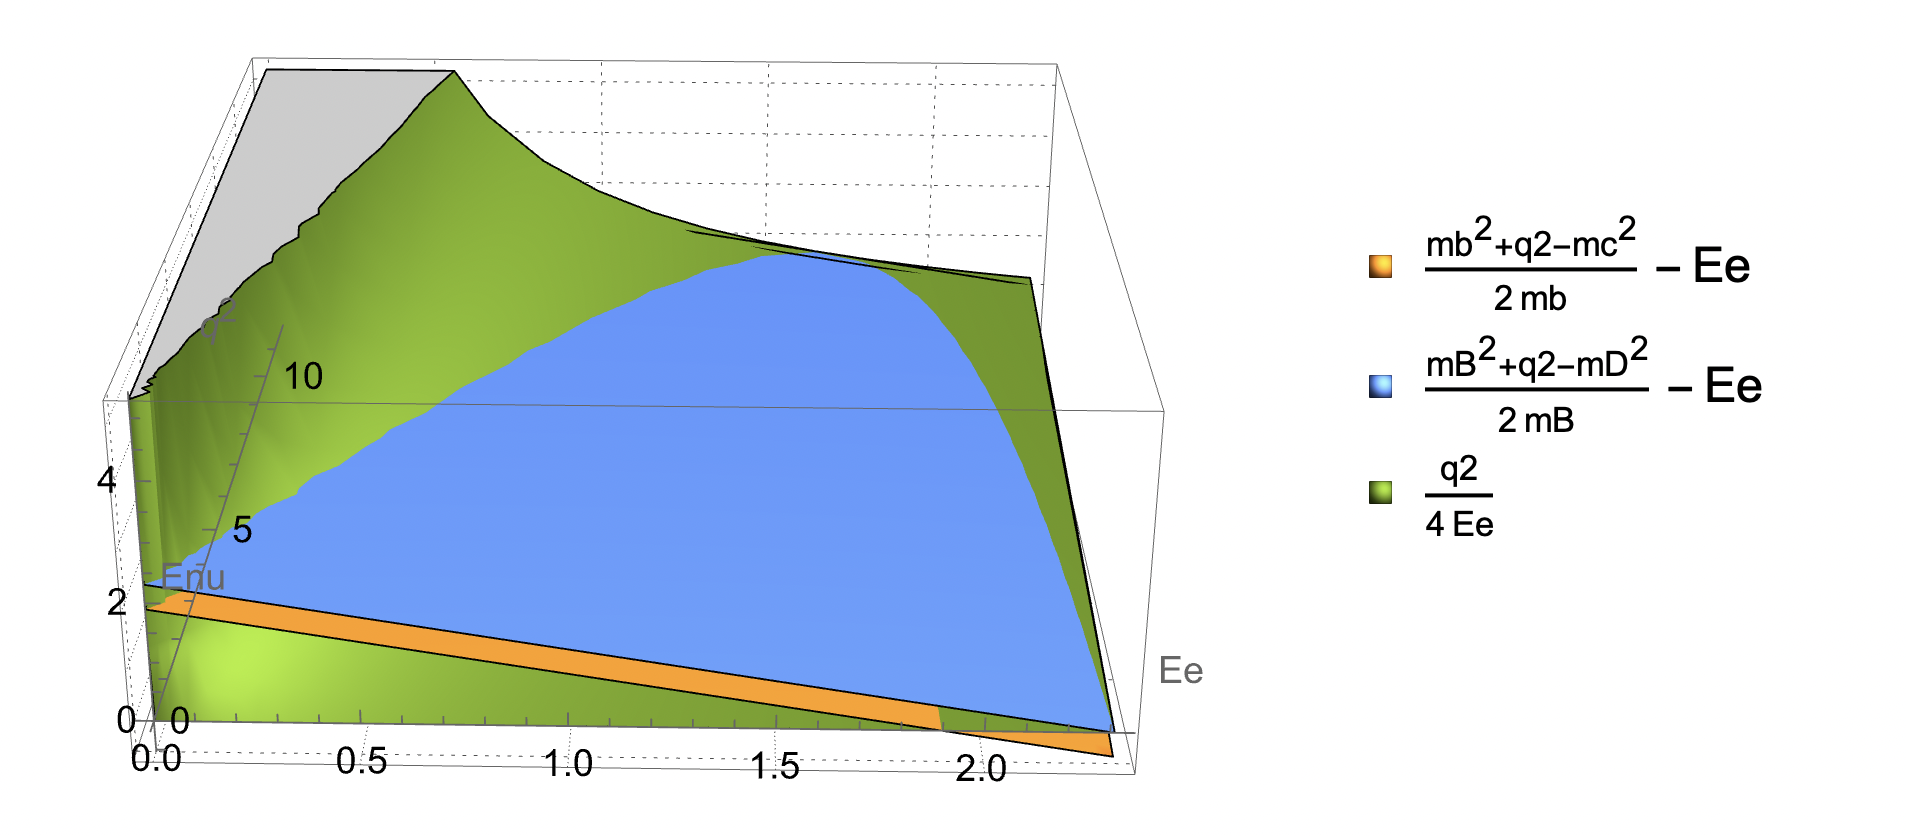
\includegraphics[width=0.8\textwidth]{figures/treephase3.png}
    \caption{中微子能量积分区域}
    \label{fig:2.2}
    \end{figure}

完成$E_\mrm{\nu}$积分后，整体留下Heavside-Theta 函数为：
\begin{equation}
    \theta(4 E_{\mathrm{e}} E_{\mrm{\nu_{e}}} - q^2) \rightarrow \theta\left(\frac{m_{\mathrm{b}}^2 + q^2 - m_{\mathrm{c}}^2}{2 m_{\mathrm{b}}} - E_{\mathrm{e}} - \frac{q^2}{4 E_{\mathrm{e}}}\right).
\end{equation}
将Heavside-Theta 函数无量纲化，可得双微分衰变宽度如下：
\begin{equation}
    \begin{aligned}
    \frac{\mathrm{d} \Gamma}{\mathrm{d} \hat{q}^2 \, \mathrm{d} y} = & \frac{\mrm{G_F^2}m_{\mathrm{c}}^5 \left| \mrm{V_{\mathrm{cb}}} \right|^2}{192 \pi^3}\left\{ \theta ( z ) \left[ 12 \left( y - \hat{q}^2 \right) \left( 1 + \hat{q}^2 - \rho - y \right) \right. \right. \\
    & - \frac{2 \lambda_1}{m_{\mathrm{c}}^2} \left( 4 \hat{q}^2 - 4 \hat{q}^2 \rho + 4 \hat{q}^4 - 3 y + 3 \rho y - 6 \hat{q}^2 y \right) \\
    & \left. - \frac{6 \lambda_2}{m_{\mathrm{c}}^2} \left( - 2 \hat{q}^2 - 10 \hat{q}^2 \rho + 10 \hat{q}^4 - y + 5 \rho y - 10 \hat{q}^2 y \right) \right] \\
    & + \frac{\delta(z)}{y^2} \left[ - \frac{2 \lambda_1}{m_{\mathrm{c}}^2} \left( 2 \hat{q}^6 + \hat{q}^4 y^2 - 3 \hat{q}^2 y^3 - \hat{q}^2 y^4 + y^5 \right) \right. \\
    & \left. - \frac{6 \lambda_2}{m_{\mathrm{c}}^2} \hat{q}^2 \left( \hat{q}^2 - y \right) \left( 5 \hat{q}^2 - 8 y + y^2 \right) \right] \\
    & \left. + \frac{\delta^{\prime}(z)}{y^3} \left[ - \frac{2 \lambda_1}{m_{\mathrm{c}}^2} \hat{q}^2 \left( y^2 - \hat{q}^2 \right)^2 \left( y - \hat{q}^2 \right) \right] \right\},
    \end{aligned}
    \end{equation}
其中，$y = \frac{2 E_{\mathrm{e}}}{m_{\mathrm{b}}}, \quad \hat{q}^2 = \frac{q^2}{m_{\mathrm{b}}^2}, \quad \rho = \frac{m_{\mathrm{c}}^2}{m_{\mathrm{b}}^2}\quad z=1+\hat{q}^2-\rho-\hat{q}^2 / y-y$ 。
\paragraph{2. 轻子对不变质量平方的积分区域}
b$\to$ c跃迁过程中，轻子对不变质量平方满足 $q^{2}\leq4E_\mrm{e}E_\mrm{\nu_{e}}$，同时在强子层次
\begin{equation}
    \begin{aligned}
    \mrm{p}_{\mathrm{X_c}}^2 & = \left(\mrm{p}_{\mathrm{B}} - q\right)^2 \\
    & = m_{\mathrm{B}}^2 - 2 (E_{\mathrm{e}} + E_{\mathrm{\nu_e}}) m_{\mathrm{B}} + q^2.
    \end{aligned}
    \end{equation}
末态强子$\mrm{H_{c}}$在壳约束可得$E_{\mrm{\nu}}$对$q^{2}$的依赖，结合$q^{2}\leq4E_\mrm{e}E_\mrm{\nu_{e}}$可得$0 < q^2 < \frac{2 E_{\mathrm{e}}}{\left(m_{\mathrm{B}} - 2 E_{\mathrm{e}}\right)} \left( m_{\mathrm{B}}^2 - 2 E_{\mathrm{e}} m_{\mathrm{B}} - m_{\mathrm{D}}^2 \right)$,
 Heavside-Theta 函数在夸克水平上，对$q^2$产生更严格的约束。
$\theta(z)$给出的约束，即$1+q^{2}-\rho-\frac{q^2}{y}-y\geq 0$。

对中微子能量做分部积分带来新的狄拉克$\delta$函数也会给出关于$q^2$位于物理边界以内的约束曲面。因此不必对轻子对不变质量平方引入额外的 Heavside-Theta 函数进行解析延拓。
对$q^2$的积分完成之后，会整体留下$\theta(1-\rho-y)$。对于狄拉克$\delta$函数以及其导函数相关的项，注意：
\begin{equation}
	\int_{-\infty}^{\infty}\delta(x)=1, \int_{-\infty}^{\infty}\delta(x-x_0)=1, \int_{0}^{1}\delta(x-x_0)=\theta(x_{0})\theta(1-x_0).
\end{equation}
以双微分衰变宽度中的$\delta(z)$项为例，
\begin{equation}
    \int_{0}^{\frac{2 E_{\mathrm{e}}}{m_{\mathrm{D}} - 2 E_{\mathrm{e}}} \left( m_{\mathrm{D}}^2 - 2 E_{\mathrm{e}} m_{\mathrm{D}} - m_{\mathrm{D}}^2 \right)} \delta\left(q^2 - \frac{y(1 - \rho - y)}{1 - y}\right) \, dq^2 = \theta(1 - \rho - y).
\end{equation}
对$q^2$积分后可得到b$\to$c过程电子能谱为：
\begin{equation}
\begin{aligned}
\frac{\mathrm{d} \Gamma}{\mathrm{d} y}= & \frac{\mrm{G_F^2} m_\mrm{b}^5\mrm{\left|V_{bc}\right|^2}}{192 \pi^3}\left\{\left[2(3-2 y) y^2-6 y^2 \rho-\frac{6 y^2 \rho^2}{(1-y)^2}+\frac{2(3-y) y^2 \rho^3}{(1-y)^3}\right]\right. \\
& -\frac{2 \lambda_1}{m_\mrm{b}^2}\left[-\frac{5}{3} y^3-\frac{y^3(5-2 y) \rho^2}{(1-y)^4}+\frac{2 y^3\left(10-5 y+y^2\right) \rho^3}{3(1-y)^5}\right] \\
& -\frac{6 \lambda_2}{m_\mrm{b}^2}\left[-y^2 \frac{(6+5 y)}{3}+\frac{2 y^2(3-2 y) \rho}{(1-y)^2}\right. \\
& \left.\left.+\frac{3 y^2(2-y) \rho^2}{(1-y)^3}-\frac{5 y^2\left(6-4 y+y^2\right) \rho^3}{3(1-y)^4}\right]\right\}\theta(1-\rho-y).
\end{aligned}
\label{eq:electron_sp}
\end{equation}
在电子能量的端点处，式\eqref{eq:electron_sp}出现严重发散\footnote{在电子能量的端点处，算符乘积展开失效，这个区域HQET的展开参数不再是一个小量，形式上表现为$\ref{eq:electron_sp}$中出现的发散项}，为了处理类似的发散，尝试对端点处的奇异项进行重求和，具有模型依赖的形状函数（shape function）被引入。此外从模型无关的角度出发可以对电子能谱进行加权积分\footnote{积分可以抹平（smearing）被积函数的奇异性。}，获得衰变宽度，电子能量矩等多种物理可观测量。
\paragraph{3. 电子能量的积分区域}
末态强子$\mrm{H_{c}}$的在壳对$q^2$的约束为
$$0 < q^2 < \frac{2 E_{\mathrm{e}}}{\left(m_{\mathrm{B}} - 2 E_{\mathrm{e}}\right)} \left( m_{\mathrm{B}}^2 - 2 E_{\mathrm{e}} m_{\mathrm{B}} - m_{\mathrm{D}}^2 \right).$$
$q^2$等于零点处的电子能量具有最大值为：
$$E_{\mathrm{e}}^{\max} = \frac{m_{\mathrm{B}}^2 - m_{\mathrm{D}}^2}{2 m_{\mathrm{B}}}.$$
此外，\begin{equation}
    E_{\mathrm{e}} = \frac{m_{\mathrm{B}}^2 - m_{\mathrm{D}}^2 - q^2}{2 m_{\mathrm{B}}} - E_{\mathrm{\nu_e}}.
\end{equation}
 当 $\mrm{X_{q}}$是最轻的含粲强子且 $q^2=0$,$E_\nu=0$，电子能量具有最大值。
 
电子能谱中的 Heavside-Theta 函数给出夸克跃迁水平上电子能量的约束$y\in [0, 1-\rho]$。显然Heavside-Theta 函数给出的约束比强子层次上的约束更严格。
对电子能量做积分可得衰变宽度为：
\begin{equation}
\begin{aligned}
\Gamma= & \frac{\mrm{G_F^2} m_\mrm{b}^5\mrm{\left|V_{bc}\right|^2}}{192 \pi^3}\left[\left(1-8 \rho+8 \rho^3-\rho^4-12 \rho^2 \ln \rho\right)\right. \\
& +\frac{\lambda_1}{2 m_\mrm{b}^2}\left(1-8 \rho+8 \rho^3-\rho^4-12 \rho^2 \ln \rho\right) \\
& \left.-\frac{3 \lambda_2}{2 m_\mrm{b}^2}\left(3-8 \rho+24 \rho^2-24 \rho^3+5 \rho^4+12 \rho^2 \ln \rho\right)\right].
\end{aligned}
\label{eq:decaywidth_B_1}
\end{equation}
上式等号右边的第一行是衰变宽度的领先幂次贡献，对应与自由夸克水平的跃迁。当$\rho\to 0$且电子能量位于端点区域时，式\eqref{eq:electron_sp}中存在发散项为： 
\begin{equation}
    g_\rho(y)=\frac{\rho^{n-1}}{(1-y)^n} \theta(1-\rho-y)\quad, n=1,2,3,\cdots.
    \end{equation}
真实物理过程的$\rho\neq 0$. 本文通过研究$g_\rho(y)$在极限情况下的渐近行为以分析电子能谱发散行为。
\begin{figure}[h!]
    \centering 
    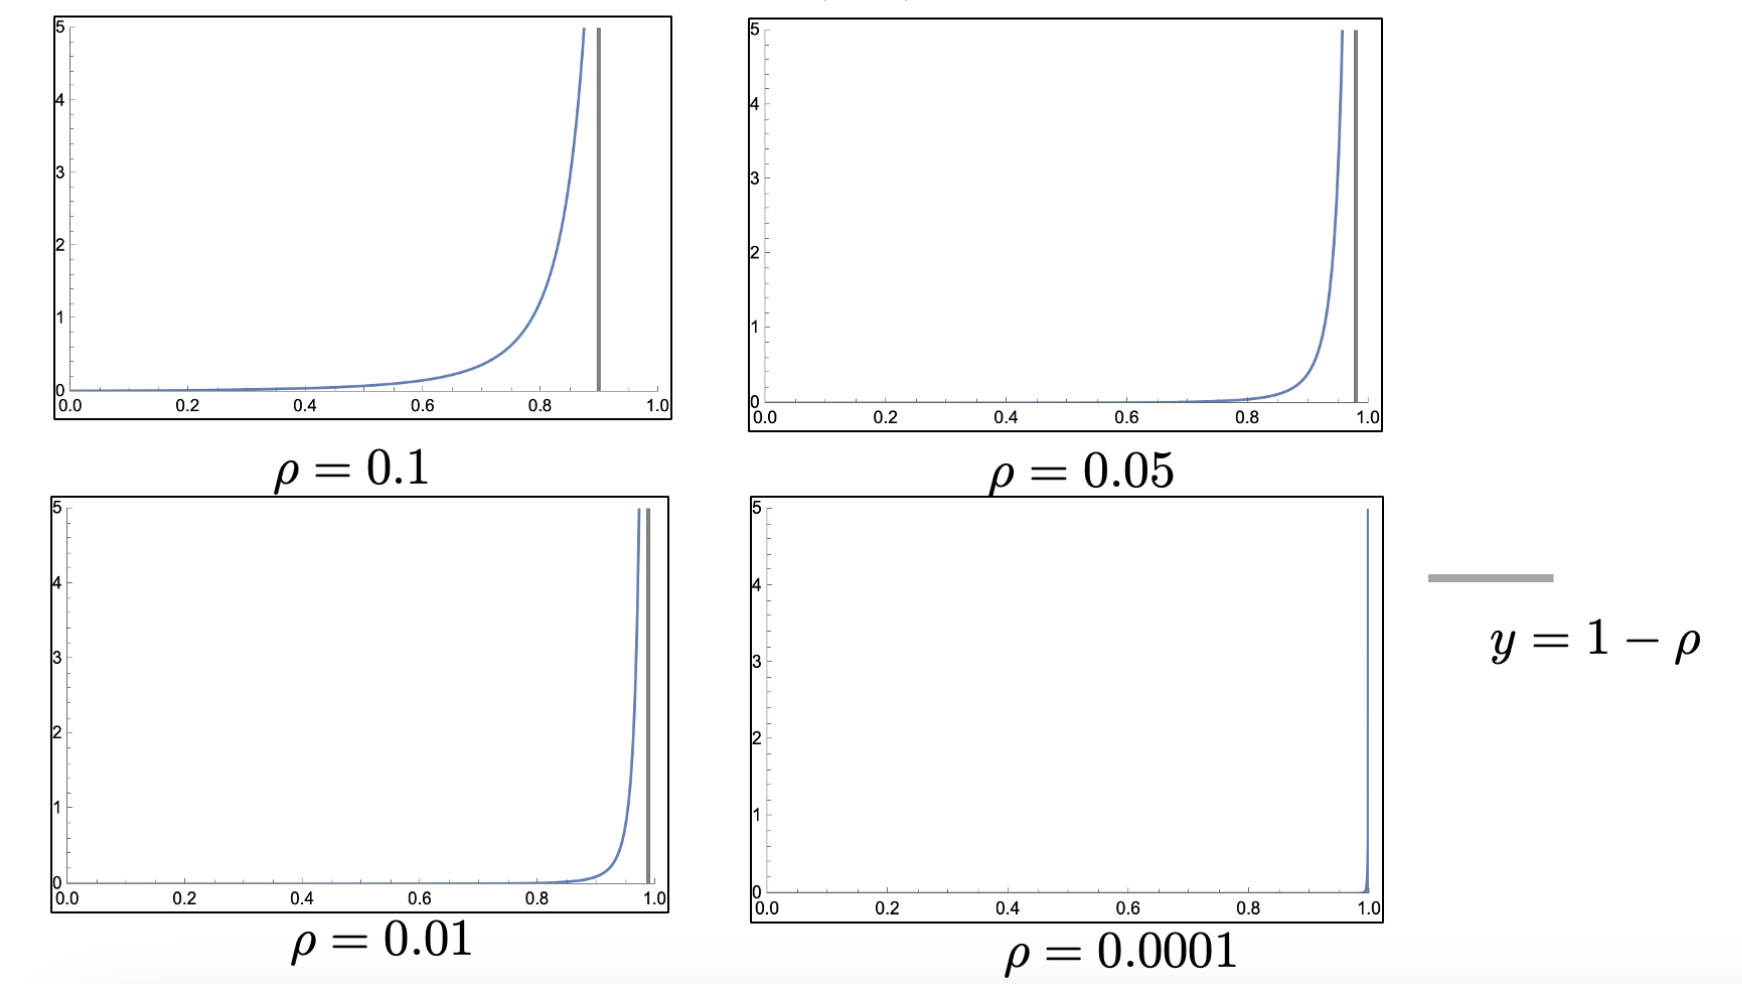
\includegraphics[width=0.8\textwidth]{figures/asymptotes.png}
    \caption{$\mrm{b\to u}$过程中电子能谱发散项的渐近行为}
    \label{fig:asp}
    \end{figure}
    本文用$\rho=0.1, 0.05, 0.01, 0.0001$为例，分析$g_\rho(y)(n=3)$的渐近行为。从图\ref{fig:asp}可知，$g_\rho(y)(n=3)$在$y=1-\rho$处发散，且发散行为处于渐近线的左侧。
    此外本文用光滑函数$t(y)$测试$g_\rho(y)$的积分行为，
    \begin{equation}
        \begin{aligned}
        \lim _{\rho \rightarrow 0} \int_0^{1-\rho} \mrm{d} y t(y) g_\rho(y) & =\frac{1}{(n-1)}\left[t(1)-\lim _{\rho \rightarrow 0} \int_0^{1-\rho} \mrm{d} y \frac{\mathrm{~d} t}{\mathrm{~d} y}(y) \frac{\rho^{n-1}}{(1-y)^{n-1}}\right] \\
        & =\frac{1}{(n-1)} t(1) .
        \end{aligned}
        \label{eq:asp_int}
        \end{equation}
    式\eqref{eq:asp_int}等号右边侧的第二项交换极限取积分次序，则被积函数等于零。最终$g_{\rho}(y)$可被等效为：
    \begin{equation}
        \begin{aligned}
        & \lim _{\rho \rightarrow 0} \frac{\rho^{n-1}}{(1-y)^n} \theta(1-\rho-y)=\frac{1}{(n-1)} \delta\left(1^{-}-y\right) \theta(1-y)=\frac{1}{(n-1)} \delta(1-y) \theta\left(1^{+}-y\right), \\
        & \lim _{\rho \rightarrow 0} \frac{\rho^{n-1}}{(1-y)^{n+1}} \theta(1-\rho-y)=-\frac{1}{(n-1)} \delta^{\prime}(1-y) \theta\left(1^{+}-y\right).
        \end{aligned}
        \label{eq:asp_replace}
        \end{equation}
    式\eqref{eq:asp_replace}中，$1^{+}$表示该值位于1的右侧领域，$1^{-}$表示该值位于1的左侧领域，结果表明$\delta$函数位于电子能量的积分区域。$\mrm{b}\to\mrm{u}$过程电子能谱为：
    \begin{equation}
        \begin{aligned}
        \frac{1}{\Gamma_0} \frac{\mathrm{~d} \Gamma}{\mathrm{~d} y}= & \left\{2(3-2 y) y^2 \theta(1-y)\right. \\
        & -\frac{2 \lambda_1}{m_\mrm{b}^2}\left[-\frac{5}{3} y^3 \theta(1-y)+\frac{1}{6} \delta(1-y) \theta\left(1^{+}-y\right)+\frac{1}{6} \delta^{\prime}(1-y) \theta\left(1^{+}-y\right)\right] \\
        & \left.-\frac{2 \lambda_2}{m_\mrm{b}^2}\left[-y^2(6+5 y) \theta(1-y)+\frac{11}{2} \delta(1-y) \theta\left(1^{+}-y\right)\right]\right\}
        \end{aligned}
        \end{equation}
    其中，$\Gamma_{0}=\frac{\left|V_{ub}\right|^2 G_F^2m_{b}^5}{192 \pi^3}$。
\subsection{第二种参数化方案}
    Andrea Albertia, Thorsten Ewerthb,等人在单圈水平上讨论了量纲五算符非微扰矩阵元对结构函数的修正\ct{Alberti:2012dn}。他们采用了一组新的运动学变量对相空间进行参数化。定义如下，
    \begin{equation}
            \hat{u}=\frac{(p-q)^2-m_{\mrm{c}}^2}{m_{\mrm{b}}^2},\quad
            \hat{q^2}=\frac{q^2}{m_{\mrm{b}}^2},\quad
            \hat{E}_{\mrm{e}}=\frac{E_{\mrm{e}}}{m_{\mrm{b}}}.\quad
        \label{eq:parameters_2}
    \end{equation}
    式\eqref{eq:parameters_2}中，$\hat{u}$是中间传播子的离壳度，在树图水平上$\hat{u}=0$.
    
    作为过渡，本节在树图水平上讨论包含量纲三算符和量纲五算符修正的电子能谱。一方面与上节结果进行交叉检验; 另一方面,本文在单圈水平上讨论量纲三算符对$\mrm{D\to X e^{+}\nu_e}$过程电子能谱的修正奠定必要的基础。

    衰变宽度关于无量纲化电子能量、轻子对转移动量平方和传播子离壳度的微分衰变宽度为：
    \begin{equation}
        \begin{aligned}
        \frac{\mathrm{d} \Gamma}{\mathrm{d} \hat{E}_{\mrm{\ell}} \, \mathrm{d} \hat{q}^2 \, \mathrm{d} \hat{u}} = & \frac{\mrm{G_F^2} m_{\mathrm{b}}^5 \left| \mrm{V_{\mathrm{cb}}} \right|^2}{16 \pi^3} \theta \left[ \frac{1}{2} \left( 1 - \rho + \hat{q}^2 - \hat{u} \right) - E_{\mathrm{e}} - \frac{\hat{q}^2}{4 E_{\mathrm{e}}} \right] \\
        & \times \left\{ \hat{q}^2 W_1 - \left[ 2 \hat{E}_{\mrm{\ell}}^2 - 2 \hat{E}_{\mrm{\ell}} \hat{q}_0 + \frac{\hat{q}^2}{2} \right] W_2 + \hat{q}^2 \left( 2 \hat{E}_{\mrm{\ell}} - \hat{q}_0 \right) W_3 \right\},
        \end{aligned}
        \label{eq:diffwidth_2}
        \end{equation}   
        其中的标量结构函数可以进行强相互作用耦合常数的微扰展开和底夸克质量负幂次的幂次展开：     
$$
W_i = W_i^{(0)} + \frac{\mu_{\mathrm{\pi}}^2}{2 m_{\mathrm{b}}^2} W_i^{(\mathrm{\pi}, 0)} + \frac{\mu_{\mathrm{G}}^2}{2 m_{\mathrm{b}}^2} W_i^{(\mathrm{G}, 0)} + \frac{C_F \alpha_s}{\pi} \left[ W_i^{(1)} + \frac{\mu_{\mathrm{\pi}}^2}{2 m_{\mathrm{b}}^2} W_i^{(\mathrm{\pi}, 1)} + \frac{\mu_{\mathrm{G}}^2}{2 m_{\mathrm{b}}^2} W_i^{(\mathrm{G}, 1)} \right]+\cdots.
$$
本节忽略高阶修正仅考虑树图水平贡献。其中树图水平上的结构函数 $W_{i}, i=1,2,3$ 为：
$$
W_i^{(0)}=w_i^{(0)} \delta(\hat{u}) ; \quad w_1^{(0)}=2 E_0, \quad w_2^{(0)}=4, \quad w_3^{(0)}=2.
$$
树图水平上量纲五算符(动力学算符)对应的的结构函数 $W_{i}^{(\pi,0)}, i=1,2,3$ 如下所示：
\begin{equation}
W_i^{(\pi, 0)}=w_i^{(\pi, 0)} \delta(\hat{u})+w_i^{(\pi, 1)} \delta^{\prime}(\hat{u})+w_i^{(\pi, 2)} \delta^{\prime \prime}(\hat{u}),
\end{equation}
$$
\begin{array}{lll}
w_1^{(\pi, 0)}=\frac{8}{3}\left(1-E_0\right), & w_1^{(\pi, 1)}=\frac{4}{3} E_0\left(1-E_0\right), & w_1^{(\pi, 2)}=\frac{2}{3} E_0 \lambda_0 ,\\
w_2^{(\pi, 0)}=0, & w_2^{(\pi, 1)}=-8\left(1-E_0\right), & w_2^{(\pi, 2)}=\frac{4}{3} \lambda_0 , \\
w_3^{(\pi, 0)}=-2, & w_3^{(\pi, 1)}=-\frac{4}{3}\left(1-E_0\right), & w_3^{(\pi, 2)}=\frac{2}{3} \lambda_0,
\end{array}
$$
树图水平上量纲五算符(色磁算符)对应的结构函数 $W_{i}^{(G,0)}, i=1,2,3$ 如下所示：
\begin{equation}
    W_i^{(\mathrm{G}, 0)} = w_i^{(\mathrm{G}, 0)} \delta(\hat{u}) + w_i^{(\mathrm{G}, 1)} \delta^{\prime}(\hat{u});
    \end{equation}
$$
\begin{array}{ll}
w_1^{(\mathrm{G}, 0)} = -\frac{4}{3} \left( 2 - 5 E_0 \right), & w_1^{(\mathrm{G}, 1)} = -\frac{4}{3} \left( E_0 + 3 E_0^2 + \frac{1}{2} \lambda_0 \right) ; \\
w_2^{(\mathrm{G}, 0)} = 0, & w_2^{(\mathrm{G}, 1)} = \frac{8}{3} \left( 3 - 5 E_0 \right) ; \\
w_3^{(\mathrm{G}, 0)} = \frac{10}{3}, & w_3^{(\mathrm{G}, 1)} = -\frac{4}{3} \left( 1 + 5 E_0 \right) .
\end{array}
$$

其中，$E_0=\frac{1}{2}\left(1+\rho-\hat{q}^2\right)$, $\lambda_0=4\left(E_0^2-\rho\right)$.

对于$(E_{\mathrm{e}}, E_{\mathrm{\nu_e}}, q^2)$这组运动学变量，$E_{\mathrm{\nu_e}}$的下限是$\frac{\hat{q^{2}}}{4 E_{\mrm{e}}}$.  当固定$E_{\mrm{e}}, q^2$, 中间传播子离壳度$\hat{u}$与中微子能量$E_{\mrm{\nu_{e}}}$存在一一对应的关系。即$$\hat{u} = 1 + \hat{q^2} - \rho - 2 \left( \hat{E_{\mathrm{e}}} + \hat{E}_{\mathrm{\nu_e}} \right).$$ $\hat{u}$的运动学区域的上限是$(1 - \rho + \hat{q^2}) - 2 \hat{E_{\mathrm{e}}} - \frac{\hat{q^2}}{2 E_{\mathrm{e}}}$，类似地,引入$$\theta\left[\frac{1}{2}(1-\rho+\hat{q^2}-\hat{u})-E_{\mrm{e}}-\frac{\hat{q^{2}}}{4 E_{\mrm{e}}}\right],$$将对积分区域解析延拓到正无穷,这是式\eqref{eq:diffwidth_2}中Heavside-theta项。
\begin{figure}[h!]
    \centering
    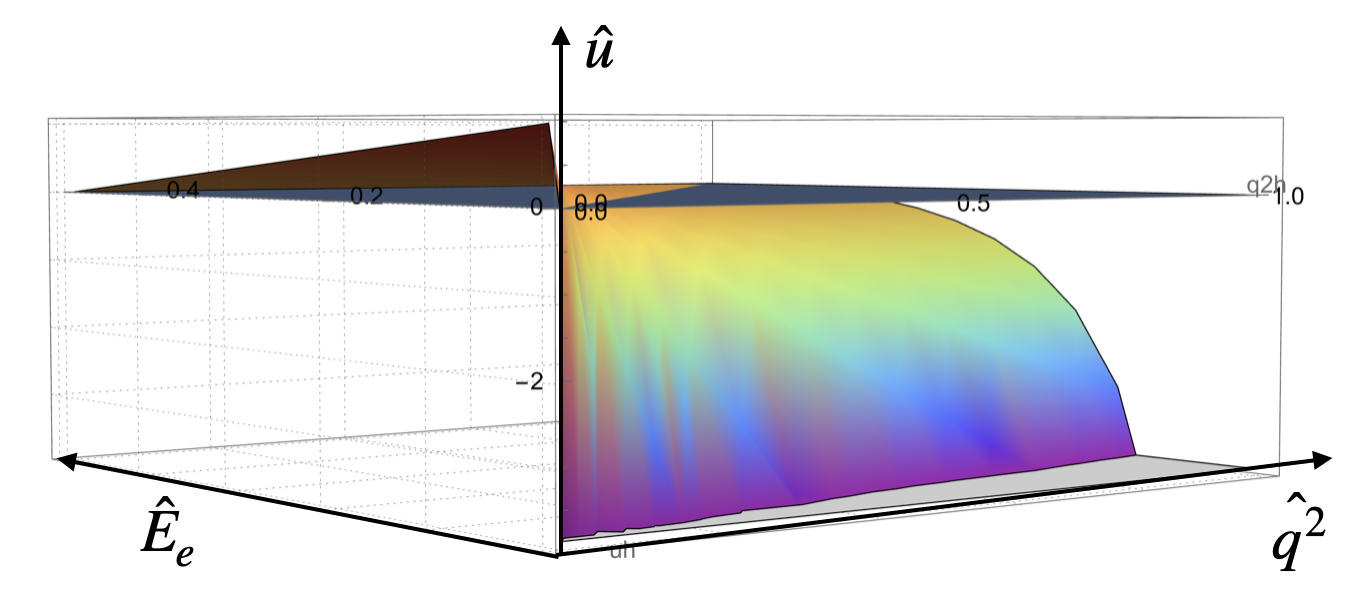
\includegraphics[width=0.8\textwidth]{figures/phase2.png}
    \caption{中间传播子离壳度的积分区域}
\end{figure}

完成对$\hat{u}$的积分\footnote{$\hat{q^{0}}$表示无量纲化的中微子能量和电子能量之和， 这时$\hat{u}=1+\hat{q^{2}}-\rho-2\hat{q^{0}}$.具体地， 树图水平对应于$\hat{u}=0$，$\hat{q^{0}}$是关于$\hat{u}$的函数，在分部积分的过程中，$\hat{q^{0}}(\hat{u})$在零点关于$\hat{u}$的导数必须在先对$\hat{q^{0}}(\hat{u})$求导，然后再取导函数在零点处的值。}, Heavside-Theta函数变成$\theta\left(\frac{(4 \hat{E}_\mrm{e} - 2 (1 - \rho)) \hat{E}_\mrm{e}}{2 \hat{E}_\mrm{e} - 1}\right)$, 这将给出关于$\hat{q^{2}}$的积分区域，完成对$\hat{q^{2}}$的积分之后，可得了$\mrm{\bar{B}}\to \mrm{X_{c}}e\nu$过程的电子能谱为：
\begin{equation}
    \begin{aligned}
        \frac{1}{\Gamma_{0}} \frac{d \Gamma}{d \hat{E}_{\mathrm{e}}} = \{ & 16 \hat{E}_{\mathrm{e}}^2 (3 - 4 \hat{E}_{\mathrm{e}}) - 48 \hat{E}_{\mathrm{e}}^2 \rho - \frac{48 \hat{E}_{\mathrm{e}}^2 \rho^2}{(1 - 2 \hat{E}_{\mathrm{e}})^2} + \frac{16 \hat{E}_{\mathrm{e}}^2 (3 - 2 \hat{E}_{\mathrm{e}}) \rho^3}{(1 - 2 \hat{E}_{\mathrm{e}})^3} \\
        & - \frac{32 \mu_{\pi}^2}{3 m_{\mathrm{b}}^2} \hat{E}_{\mathrm{e}}^3 \left[ 5 + \frac{3 (5 - 4 \hat{E}_{\mathrm{e}})}{(1 - 2 \hat{E}_{\mathrm{e}})^4} \rho^2 - \frac{4 (2 \hat{E}_{\mathrm{e}}^2 - 5 \hat{E}_{\mathrm{e}} + 5)}{(1 - 2 \hat{E}_{\mathrm{e}})^5} \rho^3 \right] \\
        & + \frac{32 \mu_{\mathrm{G}}^2}{3 m_{\mathrm{b}}^2} \hat{E}_{\mathrm{e}}^2 \left[ 3 + 5 \hat{E}_{\mathrm{e}} + \frac{3 (4 \hat{E}_{\mathrm{e}} - 3)}{(1 - 2 \hat{E}_{\mathrm{e}})^2} \rho - \frac{9 (1 - \hat{E}_{\mathrm{e}})}{(1 - 2 \hat{E}_{\mathrm{e}})^3} \rho^2 + \frac{5 (2 \hat{E}_{\mathrm{e}}^2 - 4 \hat{E}_{\mathrm{e}} + 3)}{(1 - 2 \hat{E}_{\mathrm{e}})^4} \rho^3 \right] \\
        & \} \theta \left( \frac{1 - \rho}{2} - \hat{E}_{\mathrm{e}} \right).
    \end{aligned}
\end{equation}

整体会留下另一个 Heavside-Theta函数$\theta(\frac{1-\rho}{2}-\hat{E}_{e})$对$\hat{E}_{e}$积分区域进行限制。关于无量纲化电子能量的积分，Heavside-Theta函数给出的约束是$\left[0,\frac{1-\rho}{2}\right]$,最终可得$\mrm{B\to X_{c} e\nu}$过程的衰变宽度为：
\begin{equation}
    \begin{aligned}
    \frac{\Gamma}{\Gamma_{0}}=&1 - 8 \rho + 8 \rho^3 - \rho^4 - 12 \rho^2 \ln\rho\\
    &-\mu_{\pi}^2\left[1 - 8 \rho + 8 \rho^3 - \rho^4 - 12 \rho^2 \ln\rho\right]\\
    &+\mu_{G}^2\left[3 - 8 \rho + 24 \rho^2 - 24 \rho^3 + 5 \rho^4 + 12 \rho^2 \ln\rho\right],\\
\end{aligned}
\end{equation}
该结果与式\eqref{eq:decaywidth_B_1}保持一致。
\subsection{两种参数化方案之间的转换}
为了方便两种参数化方案之间进行交叉检验，本节讨论两种参数化方案下的结构函数、微分衰变宽度和衰变宽度之间的转换关系。

\subsubsection{第一种参数化方案}
$\mrm{\bar{B}}$介子半轻单举衰变宽度为：
\begin{equation}
    \begin{aligned}
        \Gamma =  \int \frac{\mrm{d}^{3} \vec{p_{\mathrm{e}}}}{(2 \pi)^{3} 2 E_{\mathrm{e}}} &\frac{\mrm{d}^{3} \vec{p_{\mathrm{X_{c}}}}}{(2 \pi)^{3} 2 E_{\mathrm{X_{c}}}} \frac{\mrm{d}^{3} \vec{p_{\nu_{e}}}}{(2 \pi)^{3} 2 E_{\mathrm{\nu_e}}}\times\\
         &\sum_{X_{\mathrm{c}}} \sum_{\substack{\text{lepton} \\ \text{spins}}} \frac{\left|\left\langle \mrm{X_{\mathrm{c}} \mrm{e} \mrm{\bar{\nu}}_{\mathrm{e}} }\left| H_W \right| \mrm{\bar{B}} \right\rangle \right|^2}{2 m_{\mathrm{B}}} (2 \pi)^4 \delta^4\left[p_{\mathrm{B}} - \left(p_{\mathrm{e}} + p_{\mathrm{\nu_e}}\right) - p_{X_{\mathrm{c}}}\right],
    \end{aligned}
\end{equation}
经过适当的相空间积分后，可得三微分衰变宽度为：
\begin{equation}
    \frac{\mathrm{d} \Gamma}{\mathrm{d} q^2 \, \mathrm{d} E_{\mathrm{e}} \, \mathrm{d} E_{\mathrm{\nu_e}}} = \frac{1}{4} \sum_{\mrm{X}_{\mathrm{c}}} \sum_{\substack{\text{lepton} \\ \text{spins}}} \frac{\left|\left\langle\mrm{ X e \bar{v}_{\mathrm{e}} }\left| H_W \right| \mrm{\bar{B} }\right\rangle \right|^2}{2 m_{\mathrm{B}}} \delta^4 \left[ p_{\mathrm{B}} - \left( p_{\mathrm{e}} + p_{\mathrm{\nu_e}} \right) - p_{X_{\mathrm{c}}} \right] .
    \end{equation}    
其中，
\begin{equation}
    \begin{aligned}
    & \frac{1}{4} \sum_{{X_\mathrm{c}}} \sum_{\substack{\text{lepton} \\ \text{spins}}} \frac{\left|\left\langle \mrm{X_{\mathrm{c}} e \bar{\nu}_{\mathrm{e}} }\left| H_W \right| \mrm{\bar{B}} \right\rangle \right|^2}{2 m_{\mathrm{B}}} (2 \pi)^3 \delta^4 \left[ p_{\mathrm{B}} - \left( p_{\mathrm{e}} + p_{\mathrm{\nu_e}} \right) - p_{X_{\mathrm{c}}} \right] \\
    & \quad = 2 \mrm{G_F^2} \left| V_{\mathrm{c b}} \right|^2 W_{\alpha \beta} L^{\alpha \beta},
    \end{aligned}
    \end{equation}
    
其中有关强子张量$W^{\prime}$的定义如下：
\begin{equation}
W_{\alpha \beta}^{\prime}=\operatorname{Im}(\frac{\mrm{i}}{2m_{\mrm{B}}\pi} \int \mrm{d}^4 x e^{-i q \cdot x} \left\langle\mrm{\bar{B}}\left|\operatorname{T}\left[J_{\mrm{L} \alpha}^{\dagger}(x) J_{\mrm{L} \beta}(0)\right]\right|\mrm{ \bar{B}}\right\rangle)
\end{equation}
在微扰论领头阶，
\begin{equation}
    \begin{aligned}
    W_{\alpha \beta}^{\prime} = & \sum_{\mrm{X}_{\mathrm{c}}} (2 \pi)^3 \delta^4 \left( p_{\mathrm{B}} - q - p_{X_{\mathrm{c}}} \right) \frac{1}{2 m_{\mathrm{B}}} \\
    & \times \left\langle \mrm{\bar{B} }\left( p_{\mathrm{B}} \right) \left| J_\mrm{L}^{\dagger \alpha} \right| \mrm{X_{\mathrm{c}} }\left( p_{X_{\mathrm{c}}} \right) \right\rangle \left\langle X_{\mathrm{c}} \left( p_{\mrm{X_{\mathrm{c}}}} \right) \left| J_\mrm{L}^\beta \right| \mrm{\bar{B}} \left( p_{\mathrm{B}} \right) \right\rangle,
    \end{aligned}
    \end{equation}    
基于洛伦兹对称性和电荷共轭对称性，可将$W_{\alpha \beta}^{\prime}$分解为
\begin{equation}
    m_{b}W^{\prime}_{\alpha \beta}=-g_{\alpha \beta} m_{b}W^{\prime}_1+v_\alpha v_\beta m_{b}W_2^{\prime}-i \epsilon_{\alpha \beta \mu \nu} v^\mu q^\nu m_{b} W_3^{\prime}+q_\alpha q_\beta m_{b} W_4^{\prime}+\left(v_\alpha q_\beta+v_\beta q_\alpha\right)m_{b} W_5^{\prime}
\end{equation}
轻子张量约定为：
\begin{equation}
L^{\alpha \beta}=2\left(p_e^\alpha p_{v_e}^\beta+p_e^\beta p_{v_e}^\alpha-g^{\alpha \beta} p_e \cdot p_{v_e}-i \epsilon^{\eta \beta \lambda \alpha} p_{e \eta} p_{v_e \lambda}\right)
\end{equation}
强子张量和轻子张量进行洛伦兹指标缩并之后，W4和W5消失并可得三微分衰变宽度的表达式为：
\begin{equation}
    \begin{aligned}
    \frac{\mathrm{d} \Gamma}{\mathrm{d} q^2 \, \mathrm{d} E_{\mathrm{e}} \, \mathrm{d} E_{\mathrm{\nu_e}}} = & \frac{G_F^2 \left| \mrm{V}_{\mathrm{cb}} \right|^2}{2 \pi^3} \left[ W_1^{\prime} q^2 + W_2^{\prime} \left( 2 E_{\mathrm{e}} E_{\mathrm{\nu_e}} - \frac{q^2}{2} \right) \right. \\
    & \left. + W_3^{\prime} q^2 \left( E_{\mathrm{e}} - E_{\mathrm{\nu_e}} \right) \right] \theta \left( 4 E_{\mathrm{e}} E_{\mathrm{\nu_e}} - q^2 \right)
    \end{aligned}
    \end{equation}    
对上式做无量纲化处理\footnote{$m_{b}^{5}=m_{b}^{4}\cdot m_{b}$,乘积第一项来自于微分衰变宽度表达式的左边无量纲化，第二项来自于结构函数的无量纲化。注意，$4\tilde{W_{i}}^{\prime}=W_{i}$}，
\begin{equation}
    \begin{aligned}
    \frac{\mathrm{d} \Gamma}{\mathrm{d} \hat{q}^2 \, \mathrm{d} \hat{E}_{\mathrm{e}} \, \mathrm{d} \hat{E}_{\mathrm{\nu_e}}} = & \frac{G_F^2 \left| V_{\mathrm{c b}} \right|^2 m_{\mathrm{b}}^5}{2 \pi^3} \left[ \tilde{W_1}^{\prime} \hat{q}^2 + \tilde{W_2}^{\prime} \left( 2 \hat{E}_{\mathrm{e}} \hat{E}_{\mathrm{\nu_e}} - \frac{\hat{q}^2}{2} \right) \right. \\
    & \left. + \tilde{W_3}^{\prime} \hat{q}^2 \left( \hat{E}_{\mathrm{e}} - \hat{E}_{\mathrm{\nu_e}} \right) \right] \theta \left( 4 \hat{E}_{\mathrm{e}} \hat{E}_{\mathrm{\nu_e}} - \hat{q}^2 \right)
    \end{aligned}
    \label{eq2:12}
    \end{equation}    
\subsubsection{第二种参数化方案}
$\mrm{\bar{B}}\to\mrm{X_c e\nu}$过程的强子张量约定如下
\begin{equation}
    W_{\alpha \beta}=\frac{2}{\pi}\text{Im}\{\frac{i}{m_{B}} \int d^4 x e^{-i q \cdot x} \bra{\bar{B}}T\left[J_{L \alpha}^{\dagger}(x) J_{L \beta}(0)\right] \ket{\bar{B}}\}
    \end{equation}
基于洛伦兹对称性和电荷共轭对称性，$W_{\alpha\beta}$可进行如下的张量分解：
    \begin{equation}
         m_{\mrm{b}}W_{\alpha \beta}=-g_{\alpha \beta}W_1+v_\alpha v_\beta W_2-i \epsilon_{\alpha \beta \mu \nu} v^\mu q^\nu  W_3+q_\alpha q_\beta W_4+\left(v_\alpha q_\beta+v_\beta q_\alpha\right) W_5
    \end{equation}
    此外，标量结构函数关于强相互作用耦合常数的微扰展开和关于底夸克质量负幂次的幂次展开为：
    \begin{equation}
        W_i = W_i^{(0)} + \frac{\mrm{\mu_{\pi}^2}}{2 m_{\mathrm{b}}^2} W_i^{(\pi, 0)} + \frac{\mrm{\mu_{\mathrm{G}}^2}}{2 m_{\mathrm{b}}^2} W_i^{(\mathrm{G}, 0)} + \frac{C_F \alpha_s}{\pi} \left[ W_i^{(1)} + \frac{\mrm{\mu_{\pi}^2}}{2 m_{\mathrm{b}}^2} W_i^{(\pi, 1)} + \frac{\mrm{\mu_{\mathrm{G}}^2}}{2 m_{\mathrm{b}}^2} W_i^{(\mathrm{G}, 1)} \right]
        \end{equation}        
    其中的非微扰矩阵元可进行如下参数化：
    \begin{equation}
        \begin{aligned}
            \mrm{\mu_\pi^2}&=\frac{-1}{2 m_B}\left\langle\bar{B}(v)\left|\bar{b}_v(i D)^2 b_v\right| \bar{B}(v)\right\rangle,\\
            \mrm{\mu_G^2}&=-\frac{1}{6 m_B}\left\langle\bar{B}(v)\left|\bar{b}_v \frac{g_s}{2} G_{\mu \nu} \sigma^{\mu \nu} b_v\right| \bar{B}(v)\right\rangle,
        \end{aligned}
    \end{equation}
    其中，$D_\mu=\partial_\mu+i g_s G_\mu^a T^a$是协变微分算子，$\mrm{G_{\mu\nu}}$是规范场强张量，$\mrm{b_{v}}$是静止底夸克场。$\lambda_1, \lambda_2$定义于渐进HQET区域，但实际计算过程往往位于有限夸克质量态，两者的差异如下：
    $$\mrm{\mu_\pi^2=-\lambda_1}+\mathcal{O} \left(1 / m_\mrm{b}\right)\quad \mrm{\mu_G^2=3 \lambda_2}+\mathcal{O}\left(1 / m_\mrm{b}\right)$$
   
    两种参数化方案之间关于结构函数约定的全局差异如下\footnote{这里的变量替换涉及到Dirac-delta函数及其高阶导函数，需要考虑正确地处理 Delta 函数导数的所有零点并考虑额外的雅可比行列式。$n= 0，1，2$分指别至Dirac delta函数，一阶导函数，二阶导函数}：
    \begin{equation}
        \begin{aligned}
                W_{\alpha \beta}(q^{2}, \hat{u}) &= 4 \cdot 2^{n+1} (-1)^{n} W^{\prime}_{\alpha \beta}(q^{2}, q^{0}) \\
                W_{i} &= 4 m_{\mathrm{b}} \cdot 2^{n+1} (-1)^{n} W_{i}^{\prime}(q^{2}, q^{0}), \, i = 1, 2 \\
                W_{3} &= 4 m_{\mathrm{b}}^{2} \cdot 2^{n+1} (-1)^{n} W_{3}^{\prime}(q^{2}, q^{0}) \\
                W_{4} &= 4 m_{\mathrm{b}}^{3} \cdot 2^{n+1} (-1)^{n} W_{4}^{\prime}(q^{2}, q^{0}) \\
                W_{5} &= 4 m_{\mathrm{b}}^{2} \cdot 2^{n+1} (-1)^{n} W_{5}^{\prime}(q^{2}, q^{0}) \\
        \end{aligned}
    \end{equation}    
    
    $\mrm{\bar{B}\to X_{c}e\nu}$过程在新的参数化方案下的三微分衰变宽度为： 
    \begin{equation}
    \begin{aligned}
    \frac{\mrm{d} \Gamma}{\mrm{d} \hat{E}_{\mrm{\ell}} \mrm{d} \hat{q}^2 \mrm{d} \hat{u}}= & \frac{\mrm{G_F^2} m_\mrm{b}^5\mrm{\left|V_{c b}\right|^2}}{16 \pi^3} \theta\left(\hat{u}_{+}-\hat{u}\right) \times \\
    & \times\left\{\hat{q}^2 W_1-\left[2 \hat{E}_{\mrm{\ell}}^2-2 \hat{E}_{\mrm{\ell}} \hat{q}_0+\frac{\hat{q}^2}{2}\right] W_2+\hat{q}^2\left(2 \hat{E}_{\mrm{\ell}}-\hat{q}_0\right) W_3\right\},
    \end{aligned}
    \label{eq:2:23}
    \end{equation}
    从\ref{eq2:12}出发，简单讨论\ref{eq:2:23}与\ref{eq2:12}之间的一致性\footnote{不能简单地认为\ref{eq:2:24}和\ref{eq:2:25}在三微分衰变宽度上成立（尽管在树图阶的领先幂次看起来是这样）。一般地, 将三微分衰变宽度的表达式分为$\delta$项、$\delta^{\prime}$项、$\delta^{\prime\prime}$项，则\ref{eq:2:24}分别取n=0，1，2时，等号对应成立。}
    \begin{equation}
        \begin{aligned}
    \frac{\mathrm{d} \Gamma}{\mathrm{d} \hat{q}^2 \, \mathrm{d} \hat{E}_{\mathrm{e}} \, \mathrm{d} \hat{E}_{\mathrm{\nu_e}}} = & \frac{G_F^2 \left| V_{\mathrm{c b}} \right|^2 m_{\mathrm{b}}^5}{4 \cdot 2 \pi^3 \cdot 2^{n+1} (-1)^n} \left[ W_1 \hat{q}^2 + W_2 \left( 2 \hat{E}_{\mathrm{e}} \hat{E}_{\mathrm{\nu_e}} - \frac{\hat{q}^2}{2} \right) \right. \\
    & \left. + W_3 \hat{q}^2 \left( \hat{E}_{\mathrm{e}} - \hat{E}_{\mathrm{\nu_e}} \right) \right] \theta \left( 4 \hat{E}_{\mathrm{e}} \hat{E}_{\mathrm{\nu_e}} - \hat{q}^2 \right) \\
    = & \frac{G_F^2 \left| \mrm{V_{\mathrm{c b}}} \right|^2 m_{\mathrm{b}}^5}{16 \pi^3 (-2)^n} \left\{ \hat{q}^2 W_1 - \left[ 2 \hat{E}_{\ell}^2 - 2 \hat{E}_{\ell} \hat{q}_0 + \frac{\hat{q}^2}{2} \right] W_2 + \hat{q}^2 \left( 2 \hat{E}_{\ell} - \hat{q}_0 \right) W_3 \right\}
    \end{aligned}
    \label{eq:2:24}
\end{equation}
    n取0，对应结构函数里只含有Dirac delta函数（树图阶的领先幂次），这时式\eqref{eq:2:24}与式\eqref{eq:2:23}形式上保持一致。若结构函数中存在Dirac Delta函数的高阶导函数项，则做变量替换需要谨慎考虑Dirac Delta函数的零点和额外的雅各比行列式贡献。其主要思路是：从微分衰变宽度出发，用两个准两体末态相空间积分来处理三体衰变末态，积分掉多余的运动学变量，保留$\hat{E}_{\mrm{l}}$, $\hat{u}$, $q^{2}$，可得式\eqref{eq:2:23}。而式\eqref{eq2:12}的基本思路是：从衰变宽度出发，插入$E_{l}$, $E_{\nu}$, $q^{2}$的Dirac $\delta$函数，抽取出关于$E_{\mrm{l}}$,  $E_{\mrm{\nu_e}}$，$q^{2}$的微分衰变宽度。
    \begin{equation}
        \frac{\mathrm{d} \Gamma}{\mathrm{d} \hat{q}^2 \, \mathrm{d} \hat{E}_{\mathrm{e}} \, \mathrm{d} \hat{E}_{\mathrm{\nu_e}}} = \left( - \frac{1}{2} \right)^n \frac{\mrm{d} \Gamma}{d \hat{E}_{\mrm{\ell}} \, \mrm{d} \hat{q}^2 \, \mrm{d} \hat{u}}
        \label{eq:2:25}
    \end{equation}    
    \begin{equation}
        \frac{\mathrm{d} \Gamma}{\mathrm{d} \hat{q}^2 \, \mathrm{d} \hat{E}_{\mathrm{e}}} = \frac{\mrm{d} \Gamma}{ \mathrm{d} \hat{E}_{\mrm{\ell}} \,  \mathrm{d}  \hat{q}^2}
        \label{eq:2:25}
    \end{equation}    
    关于\ref{eq:2:25}\footnote{这里的$(-\frac{1}{2})^{n}$来自于Dirac delta函数中变量替换对雅各比行列式的贡献，即上Dirac delta函数的零点和额外的雅各比行列式），树图阶没有来自被积函数变量替换带来的雅各比行列式。}, 由于分部积分引入关于积分结果的冗余自由度，即存在多种等价形式的积分结果，即\footnote{\ref{eq:2:27}第二行的公式是的$f^{\prime}(y)$的意思是先做x到y的替换，再对y整体求导。另一个公式则不用考虑这个次序：$$f(x)\delta^{\prime\prime}(x-y)=f(y)\delta^{\prime\prime}(x-y)-2f^{\prime}(x)\delta^{\prime}(x-y)-f^{\prime}(x)\delta(x-y)$$这个公式是对$f(x) \delta(x-y)=f(y) * \delta(x-y)$求两次关于x的导数整理而来。}:
    \begin{equation}
    \begin{aligned}
    & f(x) \delta^{\prime}(x-y)=f(y) * \delta^{\prime}(x-y)-f^{\prime}(y) \delta(x-y) \\
    & f(x) \delta^{\prime \prime}(x-y)=f(y) * \delta^{\prime \prime}(x-y)-2 f^{\prime}(y) \delta^{\prime}(x-y)+f^{\prime \prime}(y) \delta(x-y)
    \end{aligned}
    \label{eq:2:27}
    \end{equation} 
    基于以上讨论，可实现两组参数化方案之间的检验。
\subsection{粲强子单举衰变过程的电子能谱及衰变宽度}
粲强子半轻单举衰变相比于底强子半轻单举衰变的区别在于轻子部分，前者轻子末态是正电子和电子中微子，而后者轻子末态是电子和反电子中微子。这一区别反映在轻子张量上Levi-theta项上，最终表现为微分衰变宽度中$W_{3}$项。因此本节直接给出树图水平上精确至量纲五算符非微扰矩阵元水平的$\mrm{D\to X e^{+}\nu_{e}}$过程电子能谱，
\begin{equation}
    \begin{aligned}
        \frac{1}{\Gamma_{0}} \frac{\mathrm{d} \Gamma}{\mathrm{d} \hat{E}_{\mathrm{e}}} = & 96 \hat{E}_{\mathrm{e}}^2 (1 - 2 \hat{E}_{\mathrm{e}}) \theta\left( \frac{1}{2} - \hat{E}_{\mathrm{e}} \right) \\
        & + \frac{8 \mu_{\pi}^2}{m_{\mathrm{c}}^2} \hat{E}_{\mathrm{e}}^3 \left[ 20 \hat{E}_{\mathrm{e}} + (5 - 6 \hat{E}_{\mathrm{e}}) \delta \left( \frac{1}{2}^{-} - \hat{E}_{\mathrm{e}} \right) \right] \theta\left( \frac{1}{2} - \hat{E}_{\mathrm{e}} \right) \\
        & - \frac{32 \mu_{\mathrm{G}}^2}{m_{\mathrm{c}}^2} \hat{E}_{\mathrm{e}}^2 (3 - 5 \hat{E}_{\mathrm{e}}) \theta\left( \frac{1}{2} - \hat{E}_{\mathrm{e}} \right) \\
        & + \cdots,
    \end{aligned}
    \label{eq:c_electron_sp}
\end{equation}
式\eqref{eq:c_electron_sp}中，$\hat{E}_{e}=\frac{E_{\mrm{e}}}{m_{\mrm{c}}}$, $\Gamma_{0}=\frac{\mrm{G_F^2} m_\mrm{c}^5 \mrm{V}_{\text{CKM}}}{192\pi^3}$, $\frac{1}{2}^{-}$表示该值位于1/2的左侧邻域，第一行是量纲三算符对电子能谱的贡献，第二行和第三行分别是量纲五算符$\mu_{\pi}^{2}$和$\mu_{\mrm{G}}^{2}$对电子能谱的贡献。基于该电子能谱进行加权积分，可得衰变宽度、电子能量矩等多种物理可观测量。例如衰变宽度,
\begin{equation}
    \frac{1}{\Gamma_{0}}\Gamma=1-\frac{1}{2 m_{c}^2}\mu_{\pi}^{2}-\frac{3}{2 m_{c}^2}\mu_{G}^{2}
    \label{eq:decaywidth_C_tree}
\end{equation}
式\eqref{eq:decaywidth_C_tree}中, $\mrm{V_{\text{CKM}}}$主要包含两部分，即$\mrm{V_{\text{cs}}}$和$\mrm{V_{\text{cd}}}$,末态夸克质量取零极限对应于$\mrm{c\to d}$跃迁；对于$\mrm{c\to s}$跃迁，由于奇异夸克质量并非特别小，需要作为软自由度进行保留。本文采用Mannel等人的结果\ct{Fael:2019umf}来考虑末态有限夸克质量效应对粲强子半轻单举衰变的修正。
\section{微扰修正}
本节讨论$\mrm{D\to X e^{+}\nu_{e}}$过程单圈水平上领先幂次的修正：从$\mrm{B\to X_{\text{c}}e\nu}$过程的领先幂次出发，取末态夸克零质量极限可得$\mrm{B\to X_{\text{u}}e\nu}$过程的结构函数。此外讨论$\mrm{B\to X_{\text{u}}e\nu}$的相空间解析积分，得到$\mrm{B\to X_{\text{u}}e\nu}$过程的电子能谱。基于粲强子与底强子单举衰变的区别，可得粲强子单举衰变的电子能谱。由于重夸克展开在电子能量末端失效，因此需要对电子能谱进行加权积分，得到衰变宽度、电子能量矩等各种具有非微扰参数依赖的物理量。

\subsection{单圈水平上$\mrm{B\to X_{\text{c}}e\nu}$过程的领先幂次修正}
$\mrm{B\to X_{\text{c}}e\nu}$过程的微分衰变宽度是
\begin{equation}
    \begin{aligned}
    \frac{\mathrm{d} \Gamma}{\mathrm{d} \hat{E}_{\ell} \, \mathrm{d} \hat{q}^2 \, \mathrm{d} \hat{u}} = & \frac{G_F^2 m_{\mathrm{b}}^5 \left| \mrm{V}_{\mathrm{c b}} \right|^2}{16 \pi^3} \\
    & \times \left\{ \hat{q}^2 W_1 - \left[ 2 \hat{E}_{\ell}^2 - 2 \hat{E}_{\ell} \hat{q}_0 + \frac{\hat{q}^2}{2} \right] W_2 + \hat{q}^2 \left( 2 \hat{E}_{\ell} - \hat{q}_0 \right) W_3 \right\} \\
    & \times \theta \left[ \frac{1}{2} \left( 1 - \rho + \hat{q}^2 - \hat{u} \right) - \hat{E}_{\mathrm{e}} - \frac{\hat{q}^2}{4 \hat{E}_{\mathrm{e}}} \right],
    \end{aligned}
\end{equation}
其中，$W_{i}, i=1, 2, 3$是该过程标量结构函数，它可以被强相互作用耦合常数与底夸克质量负幂次进行双重展开，
\begin{equation}
    W_i = W_i^{(0)} + \frac{\mu_{\pi}^2}{2 m_{\mathrm{b}}^2} W_i^{(\pi, 0)} + \frac{\mu_{\mathrm{G}}^2}{2 m_{\mathrm{b}}^2} W_i^{(\mathrm{G}, 0)} + \frac{\alpha_s}{\pi} \left[ \left[ C_F W_i^{(1)} \right] + C_F \frac{\mu_{\pi}^2}{2 m_{\mathrm{b}}^2} W_i^{(\pi, 1)} + \frac{\mu_{\mathrm{G}}^2}{2 m_{\mathrm{b}}^2} W_i^{(\mathrm{G}, 1)} \right]+\cdots,
\end{equation}
其中，$W_{i}^{(1)}$可由在单圈水平上完整理论和有效理论之间的算符匹配得到。该匹配过程基于图\ref{fig:Matching_NLO}完成，
\begin{figure}[h!]
    \centering
    
\includegraphics[width=0.7\textwidth]{MatchingNLO.png}
    \caption{两点关联函数的单圈修正\ct{Aquila:2005hq}}
    \label{fig:Matching_NLO}
\end{figure}

P. Gambino等人05年的工作中\ct{Aquila:2005hq}, 讨论了$\mrm{B\to X_{\text{c}}e\nu}$单圈水平上领先幂次对结构函数的修正:
\begin{equation}
    W_i^{(1)}=w_i^{(0)}\left\{S_i \delta(\hat{u})-2\left(1-E_0 I_1\right)\left[\frac{1}{\hat{u}}\right]_{+}+\frac{\theta(\hat{u})}{(\rho+\hat{u})}\right\}+R_i \theta(\hat{u}),
    \end{equation}
其中， $S_i=S+\Delta_i$，
$S=2 E_0\left(I_{2,0}-I_{4,0}\right)-1-\frac{1-\rho-6 \hat{q}^2}{4 \hat{q}^2} \ln \rho-\frac{(1-\rho)^2-6 \hat{q}^2(1+\rho)+5\left(\hat{q}^2\right)^2}{4 \hat{q}^2} I_{1,0},$
$$\Delta_1=-\frac{\rho}{E_0} I_{1,0} ; \quad \Delta_2=\frac{1-\rho}{4 \hat{q}^2} \ln \rho+\left(\frac{(1-\rho)^2}{4 \hat{q}^2}-\frac{1+\rho}{4}\right) I_{1,0} ; \quad \Delta_3=0,$$
$$
I_1=\int_0^1 d y \frac{1}{\chi(y)}=\frac{\ln \frac{1+t}{1-t}}{\sqrt{\lambda}}, \quad I_{1,0}=\int_0^1 d y \frac{1}{\bar{\chi}(y)}=\frac{\ln \frac{1+t_0}{1-t_0}}{\sqrt{\lambda_0}},
$$
$$
\begin{aligned}
I_{4,0}= & \int_0^1 d y \frac{\ln \bar{\chi}(y)}{\bar{\chi}(y)}=\frac{1}{t_0 E_0}\left[\operatorname{Li}_2\left(a_1\right)-\mathrm{Li}_2\left(a_2\right)\right. \\
& \left.+\ln \frac{1+t_0}{1-t_0} \ln E_0\left(1-t_0\right)^{\frac{1}{4}}\left(1+t_0\right)^{\frac{3}{4}}+\ln E_0\left(1+t_0\right) \ln \frac{1-E_0\left(1-t_0\right)}{1-E_0\left(1+t_0\right)}\right],
\end{aligned}
$$
$$
I_{2,0}=\int_0^1 d y \frac{\ln (1-y)}{\bar{\chi}(y)}=\frac{\operatorname{Li}_2\left(1-E_0\left(1+t_0\right)\right)-\mathrm{Li}_2\left(1-E_0\left(1-t_0\right)\right)}{\sqrt{\lambda_0}},
$$
其中， $a_1=\frac{2 t_0 /\left(1+t_0\right)}{1-E_0\left(1-t_0\right)}, \quad a_2=\frac{2 t_0 E_0}{1-E_0\left(1-t_0\right)}$，$E_0=\frac{1}{2}\left(1+\rho-\hat{q}^2\right)$，$\lambda=4\left(\hat{q}_0^2-\hat{q}^2\right)=4\left(E^2-\rho-\hat{u}\right)$， $\lambda_0=4\left(E_0^2-\rho\right)$， $t=\frac{\sqrt{\lambda}}{2 E}, \quad t_0=\frac{\sqrt{\lambda_0}}{2 E_0}$，$E_0=\frac{1}{2}\left(1+\rho-\hat{q}^2\right)$.
对于实发射部分$R_{i}$，其具体解析形式为：
$$
\begin{aligned}
R_1\left(\hat{q}^2, \hat{u}\right)= & \frac{\hat{u}(3 \hat{u}+2 \rho)+\omega(3 \hat{u}+4 \rho)}{4(\hat{u}+\rho)^2}+\frac{\hat{u}^2(\omega-\hat{u})}{2(\hat{u}+\rho) \lambda_b}+\frac{6 \hat{u}}{\lambda_b} \\
& +\frac{4 \hat{u}^2-\left(6 \hat{\omega}+\lambda_b\right) \hat{u}+2 \lambda_b \hat{\omega}}{2 \lambda_b \sqrt{\lambda_b}} \log \tau, \\
R_2\left(\hat{q}^2, \hat{u}\right)= & \frac{2\left[\hat{\omega} \hat{u}(8-9 \hat{u})-8 \hat{\omega}^3+15 \hat{\omega}^2 \hat{u}+2 \hat{u}\left(\hat{u}^2-8 \hat{u}+8\right)\right]}{\lambda_b{ }^2}+\frac{64(1+\hat{\omega}-\hat{u}) \rho}{\lambda_b{ }^2} \\
& +\frac{\hat{\omega} \hat{u}(\hat{\omega}-\hat{u})^3}{\lambda_b{ }^2(\hat{u}+\rho)^2}-\frac{2\left(2 \hat{\omega}^4+\hat{\omega}^2 \hat{u}(7+4 \hat{u})-5 \hat{\omega}^3 \hat{u}-9 \hat{\omega} \hat{u}^2+2 \hat{u}^3-\hat{\omega} \hat{u}^3\right)}{\lambda_b{ }^2(\hat{u}+\rho)} \\
& +\frac{2}{\lambda_b^2 \sqrt{\lambda_b}}\left[2 \lambda_b{ }^2+\lambda_b\left(26 \hat{u}-2 \hat{u}^2+\hat{\omega}(8+3 \hat{u})+16 \rho\right)\right. \\
& \left.-6 \hat{u}\left(3 \hat{u}^2+2 \hat{u}(\rho-5)-12 \rho-\hat{\omega}(3+4 \hat{u}+3 \rho)\right)\right] \log \tau,
\end{aligned}
$$
$$
\begin{aligned}
R_3\left(\hat{q}^2, \hat{u}\right)= & -\frac{(\hat{\omega}-2) \hat{u}-\hat{\omega}^2-4(\hat{\omega}+\rho)+\lambda_b}{\lambda_b \sqrt{\lambda_b}} \log \tau-\frac{\rho}{2(\hat{u}+\rho)^2} \\
& -\frac{3 \hat{\omega}+\rho}{2(\hat{\omega}+\rho)(\hat{u}+\rho)}-\frac{8 \hat{\omega}+5 \hat{\omega}^2-3 \hat{\omega} \hat{u}+4 \rho+4 \hat{\omega} \rho-2 \hat{u} \rho}{\lambda_b(\hat{\omega}+\rho)},
\end{aligned}
$$
其中，$\tau=\frac{\hat{\omega}-\hat{u}+\sqrt{\lambda_b}}{\hat{\omega}-\hat{u}-\sqrt{\lambda_b}}$，$\hat{\omega}=\hat{q}^2-1-\rho=-\omega-\rho$, $\lambda_{b}=\lambda$.
此外，引入Plus Distribution以孤立出红外发散和共线发散是必要的，Plus Distribution定义如下，
\begin{equation}
    \int f(\hat{u})\left[\frac{1}{\hat{u}}\right]_{+} d \hat{u}=\int_0^1 \frac{f(\hat{u})-f(0)}{\hat{u}} d \hat{u}.
    \label{eq:pb_def}
    \end{equation}
在取末态夸克质量为零$(\rho\to 0)$的过程中，在结构函数的层面上会出现类似于$\ln \rho$和$\ln \rho^2$项，这类对数发散会在对$\hat{u}$做积分的时候出现。原则上有效理论是红外安全的，表现为对$\hat{u}$的相空间积分之后的结果是有限值。因此在$\rho\to 0$的过程中可以将所有红外发散或共线发散的点借助Plus Distrubution孤立出来并验证相消，基于此便可得末态夸克无质量极限下的结构函数。
\subsection{单圈水平上$\mrm{B\to X_{u}e\nu}$过程的领先幂次修正： 结构函数}
考虑关于$\hat{u}$的光滑函数$f(\hat{u})$,本节以$W_{3}^{(1)}$为例讨论
\begin{equation}
    \int f(\hat{u}) W_i^{(1)}\left(\hat{u}, \hat{q}^2\right) d \hat{u}
    \end{equation}
的积分行为，分析发散项并给出末态夸克无质量极限下的结构函数。其中，
\begin{equation}
    W_i^{(1)}=w_i^{(0)}\left\{S_i \delta(\hat{u})-2\left(1-E_0 I_1\right)\left[\frac{1}{\hat{u}}\right]_{+}+\frac{\theta(\hat{u})}{(\rho+\hat{u})}\right\}+R_i \theta(\hat{u}),
    \end{equation}
\paragraph{$\delta$项的系数} 对$I_{l,0},l=1,2,4$在$\rho=0$处泰勒展开并保留至领头项：
\begin{equation}
    \begin{aligned}
    & I_{1,0}=\frac{2 \ln \left(1-\hat{q}^2\right)-\ln \rho}{1-\hat{q}^2}+O(\rho), \\
    & I_{2,0}=\frac{\operatorname{Li}_2\left(\hat{q}^2\right)-\frac{\pi^2}{6}}{1-\hat{q}^2}+O(\rho), \\
    & I_{4,0}=\frac{2 \ln ^2\left(1-\hat{q}^2\right)+2 \operatorname{Li}_2\left(\hat{q}^2\right)-\frac{1}{2} \ln ^2 \rho}{1-\hat{q}^2}+O(\rho),
    \end{aligned}
    \end{equation}
将其带入$S$的表达式，保留至$\rho$的领先幂次，有
\begin{equation}
    S=\frac{\ln \rho}{4}+\frac{\ln ^2 \rho}{2}-\frac{\pi^2}{6}-\mathrm{Li}_2\left(\hat{q}^2\right)-2 \ln ^2\left(1-\hat{q}^2\right)-1-\frac{1-5 \hat{q}^2}{2 \hat{q}^2} \ln \left(1-\hat{q}^2\right)+O(\rho),
    \end{equation}
这里出现的类似于$\ln \rho^2$之类的项，将与其他项的系数相互抵消，最终结构函数里没有对数发散项。
\paragraph{实发射部分: $R_{3}$}  包括且不限于$W_{3}$的实发射部分，均存在这样的一般形式，即$$R_i=\frac{r_i^{(1)} \hat{u}+r_i^{(2)} \rho}{(\hat{u}+\rho)^2}+\frac{s_i}{\hat{u}+\rho}+t_i,i=1, 2, 3.$$
其中，$r_{i}^{(1)}, s_{i}^{(1)}, t_{i}^{(1)}$均关于$\hat{u}$光滑。对于$W_{3}$，有
\begin{equation}
        r_{3}^{(1)}=0,\quad
        r_{3}^{(2)}=1/2,\quad
        s_{3}=-3/2-\rho/\omega,\quad
\end{equation}
$$ t_{3}=\frac{3 \hat{u}+5 \omega -8}{\tilde{\lambda }}+\frac{\left(\tilde{\lambda }-\hat{u} \omega -2 \hat{u}-\omega ^2+4 \omega \right)}{\tilde{\lambda }}\mathcal{I}_1,$$
其中，
\begin{equation}
    \begin{aligned}
        \mathcal{I}_1&=\frac{1}{\sqrt{\tilde{\lambda}}} \ln \frac{\hat{u}+w+\sqrt{\tilde{\lambda}}}{\hat{u}+w-\sqrt{\tilde{\lambda}}},\\
        \tilde{\lambda}&=(\hat{u}+\omega)^2-4 \hat{u},\\
    \end{aligned}
    \end{equation}
$r_{3}^{(1)},r_{3}^{(2)}, s_{3}$将参与到共线发散和红外发散的相消中。下面以关于$\hat{u}$光滑的测试函数为例逐项分析其关于$\hat{u}$积分行为，
\begin{equation}
    \int_0^1 f(\hat{u}) \frac{1}{\hat{u}+\rho} d \hat{u}=\int_0^1 \frac{f(\hat{u})-f(0)+f(0)}{\hat{u}+\rho} d \hat{u}=\int_0^1 f(\hat{u})\left(\left[\frac{1}{\hat{u}}\right]_{+}-\ln \rho \delta(\hat{u})\right) d \hat{u}+O(\rho),
    \label{eq:pd1}
\end{equation}
对于$\frac{1}{\hat{u}+\rho}$项，积分意义上如下的等效是合法且必要的，
$$
\frac{1}{\hat{u}+\rho} \rightarrow\left[\frac{1}{\hat{u}}\right]_{+}-\ln \rho \delta(\hat{u}).
$$
\begin{equation}
    \int_0^1 \frac{\rho}{(\hat{u}+\rho)^2} d \hat{u}=\frac{1}{1+\rho}=1+O(\rho),
    \label{eq:pd2}
\end{equation}
对于$\frac{\rho}{\hat{u}+\rho}$项，积分意义上如下的等效是合法且必要的，
    $$
\frac{\rho}{(\hat{u}+\rho)^2} \rightarrow \delta(\hat{u}).
$$
对于$\frac{\hat{u}}{\hat{u}+\rho}$可被上面两项进行线性表出，
\begin{equation}
    \begin{aligned}
    \frac{\hat{u}}{(\hat{u}+\rho)^2} & =c_1 \frac{1}{\hat{u}+\rho}+c_2 \frac{\rho}{(\hat{u}+\rho)^2} \\
    & =\frac{c_1 \hat{u}+\left(c_1+c_2\right) \rho}{(\hat{u}+\rho)^2} \Rightarrow c_1=1, c_2=-c_1=-1,
    \end{aligned}
    \label{eq:pd3}
\end{equation}
换而言之，对于$\frac{\hat{u}}{(\hat{u}+\rho)^2}$，积分意义上如下的等效是合法且必要的，
$$
\frac{\hat{u}}{(\hat{u}+\rho)^2}\rightarrow\left[\frac{1}{\hat{u}}\right]_{+}-\ln \rho \delta(\hat{u})-\delta(\hat{u}).
$$

分析标量结构函数在积分意义上的积分行为并引入PLus Distribution分布将象征红外发散和共线发散的项（$\ln\rho$等）孤立出来。以上讨论为进一步分析红外发散和共线发散在相空间积分意义上的相消奠定了基础。对上述结果进行整理，借助Plus Distribution从实发射部分$R_{3}$中孤立出来的发散项\footnote{$\delta(\hat{u})$在关于$\hat{u}$积分的意义上不属于发散项}包括；
\begin{equation}
    (-3/2-\rho/\omega)\ln\rho \delta(\hat{u}).
\end{equation}
\paragraph{Plus Distribution部分}
关于$\hat{u}$的奇点隐藏在积分$I_{1}$和$I_{1，0}$中，由Plus Distribution的定义（式\eqref{eq:pb_def}）可得关于这部分的讨论聚焦于
\begin{equation}
    \frac{I_1-I_{1,0}}{\hat{u}},
    \label{eq:sing11}
    \end{equation}
式\eqref{eq:sing11}在$\hat{u}=\hat{q^2}=0$处是不解析的，为了明确这一点，将式$\ref{eq:sing11}$在$\omega>>\hat{u},\hat{q^{2}}$处进行展开\footnote{对于$\mathcal{I}_1$而言，展开参数是$x=2(\rho+\hat{u})/\omega$;对于$\mathcal{I}_{1,0}$而言，展开参数是$y=2\hat{u}/\omega$； 由于$0<\omega<1$，保留$(\rho+\hat{u})/\omega^2$项是必要的}。
奇异部分是
\begin{equation}
    \left.\frac{I_1-I_{1,0}}{\hat{u}}\right|_{sing}=\frac{\ln \frac{\rho}{\hat{u}+\rho}}{\omega \hat{u}} .
    \end{equation}
减除掉奇异的部分是关于$\rho$正规的，因此可以将\ref{eq:sing11}写成两部分，
\begin{equation}
    \frac{I_1-I_{1,0}}{\hat{u}}=\frac{1}{\omega\hat{u}} \ln \frac{\rho}{\hat{u}+\rho}+B\left(\hat{q}^2, \hat{u}\right)+\mathcal{O}(\rho) .
    \end{equation}
其中，
    \begin{equation}
        B(\hat{q}^2, \hat{u})=\frac{\ln(\hat{u} / \omega^2)+\omega\mathcal{I}_1}{\omega \hat{u}} \simeq \frac{\omega-2}{\omega^3} \ln \frac{\hat{u}}{\omega^2}+\frac{2(\omega-1)}{\omega^3}+\mathcal{O} (\hat{u}),
        \label{eq:B}
        \end{equation}
    式\eqref{eq:B}中仅存在关于$\hat{u}$的对数奇点，这是可积的。使用玩具模型(Toy-Model)将相关发散项孤立出来之后预备相消。将上述结论应用于实际情况，即：
    \begin{equation}
        \begin{aligned}
        & \int f(\hat{u}) I_1\left[\frac{1}{\hat{u}}\right]_{+} d \hat{u}=\int_0^1 \frac{f(\hat{u}) I_1(\hat{u})-f(0) I_{1,0}}{\hat{u}} d \hat{u} \\
        & =\underbrace{f(0) \int_0^1 \frac{I_1-I_{1,0}}{\hat{u}} d \hat{u}}_{\text{第一项}}+\underbrace{\int_0^1 \frac{(f(\hat{u})-f(0))\left(I_1-I_{1,0}\right)}{\hat{u}} d \hat{u}}_{\text{第二项}}+\underbrace{I_{1,0} \int_0^1 \frac{f(\hat{u})-f(0)}{\hat{u}} d \hat{u}}_{\text{第三项}}.
        \end{aligned}
        \label{eq:pbexplict}
        \end{equation}
        对于第一项，\begin{equation}
            \begin{aligned}
            f(0) \int_0^1 \frac{I_1-I_{10}}{\hat{u}} d \hat{u} & =f(0) \int_0^1 \frac{1}{w \hat{u}} \ln \frac{\rho}{\hat{u}+\rho} d \hat{u}+f(0) \int_0^1 B\left(\hat{q}^2, \hat{u}\right) d \hat{u} \\
            & =f(0) \cdot\left(\frac{-\frac{\pi^2}{3}+\ln ^2 \rho}{2 w}\right)+f(0) \int_0^1 B\left(\hat{q}^2, \hat{u}\right) d \hat{u}.
            \end{aligned}
            \end{equation}
        对于第二项，
        \begin{equation}
            \begin{aligned}
             \int_0^1 \frac{f(\hat{u})-f(0)}{\hat{u}}\left(I_1-I_{10}\right) d \hat{u}&=\int_0^1(f(\hat{u})-f(0))\left(\frac{1}{\omega \hat{u}} \ln \frac{\rho}{\hat{u}+p}+B\left(\hat{q}^2, \hat{u}\right)\right) d \hat{u} \\
            &=\frac{1}{w \hat{u}} \ln \frac{\rho}{\hat{u}}+O(\rho). \\
            \end{aligned}
            \end{equation}
        对于第三项，
        \begin{equation}
            I_{1,0} \int_0^1 \frac{f(\hat{u})-f(0)}{\hat{u}} d u  =\frac{2 \ln \omega}{\omega} \int_0^1 f(\hat{u})\left[\frac{1}{\hat{u}}\right]_{+} d \hat{u}-\frac{\ln \rho}{\omega} \int_0^1 f(x)\left[\frac{1}{\hat{u}}\right]_{+} d \hat{u}.
            \end{equation}
        将上面三项合并，整理可得，
        \begin{equation}
            \int f(\hat{u}) I_1\left[\frac{1}{\hat{u}}\right]_{+} d \hat{u}=\int f(\hat{u})\left[a \delta(\hat{u})+b\left[\frac{\ln \hat{u}}{\hat{u}}\right]_{+}+c\left[\frac{1}{\hat{u}}\right]_{+}+d \theta(\hat{u})\right] d \hat{u}.
            \end{equation}
        其中，$a=-\frac{\frac{\pi^2}{3}+\ln ^2 \rho}{2 w}, \quad b=-\frac{1}{w}, \quad c=\frac{2 \ln w}{w}, \quad d = B\left(\hat{q}^2, \hat{u}\right)$. 结果表明，对于任意关于$\hat{u}$光滑的积分测试函数$f(\hat{u})$, 式\eqref{eq:pbexplict}中第一、二、三项之间将发散项均可相互抵消，结果表明关于$\rho$是可积的。综上所述，最终结构函数中有关$\rho$的奇异项全部给抵消，可得$\mrm{B\to X_{u}e\nu_{e}}$的结构函数如下所示，
        \begin{equation}
            W_i^{(1)}=w_i^{(0)}\left\{\mathcal{S}_i \delta(\hat{u})-\left[\frac{\ln \hat{u}}{\hat{u}}\right]-\left(\frac{7}{4}-2 \ln w\right)\left[\frac{1}{\hat{u}}\right]+w B\left(\hat{q}^2, \hat{u}\right) \theta(\hat{u})\right\}+\mathcal{R}_i^{(1)} \theta(\hat{u}).
            \end{equation}
    其中，
            \begin{equation}
                \begin{aligned}
                &\mathcal{S}_i=-\frac{5}{4}-\frac{\pi^2}{3}-\operatorname{Li}_2(1-w)-2 \ln ^2 w-\frac{5 w-4}{2(1-w)} \ln w+\frac{\ln w}{2(1-w)} \delta_{i 2}
                \end{aligned}
                \end{equation}
            特别的，实发射部分如下所示，
            \begin{equation}
                \begin{aligned}
                \mathcal{R}_1^{(1)}= & \frac{3}{4}+\frac{\hat{u}(12-w-\hat{u})}{2 \tilde{\lambda}}+\left(w+\frac{\hat{u}}{2}-\frac{\hat{u}(2 \hat{u}+3 w)}{\tilde{\lambda}}\right) \mathcal{I}_1 \\
                \mathcal{R}_2^{(1)}= & \frac{6 \hat{u}\left(\hat{u}^2-(3-w) \hat{u}-12+13 w\right)}{\tilde{\lambda}^2}+\frac{\hat{u}-38+21 w}{\tilde{\lambda}} \\
                & -4 \frac{\frac{w}{\frac{2}{2}} \hat{u}^3+\left(2 w^2-6\right) \hat{u}^2+\left(7-3 w+\frac{5}{2} w^2\right) w \hat{u}+w^3(w-4)}{\tilde{\lambda}^2} \mathcal{I}_1 \\
                \mathcal{R}_3^{(1)}= & \frac{3 \hat{u}-8+5 w}{\tilde{\lambda}}+\frac{\hat{u}^2-(6-w) \hat{u}+4 w}{\tilde{\lambda}} \mathcal{I}_1
                \end{aligned}
                \end{equation}
上述讨论结果与Paolo Gambino等人的工作\ct{Capdevila:2021vkf}保持一致。
\subsection{单圈水平上$\mrm{B\to X_{u}e\nu}$过程的领先幂次修正： 相空间解析积分}

末态相空间解析积分的过程中，$\{\hat{u}, \hat{q^2}, \hat{E}_{e}\}$的积分区域与树图阶的讨论一致，积分思路基本如下：微分衰变宽度中包含三部分的贡献，分别是$W_{i},i=1,2,3$相关项。这里对三部分分别积分，对于某些行为复杂的函数，单独提取出来，将三部分对应的项加和之后进行积分。本节重点展示部分内容的积分流程。
\paragraph{Plus Distribution} 以$\left[\frac{1}{\hat{u}}\right]_{+}$为例，关于$\hat{u}$的解析积分为：
\begin{equation}
    \begin{aligned}
    & \int f(\hat{u}) \theta \left[ \frac{1}{2} \left( 1 + \hat{q}^2 - \hat{u} \right) - \hat{E}_{\mathrm{e}} - \frac{\hat{q}^2}{4 \hat{E}_{\mathrm{e}}} \right] \left[ \frac{1}{\hat{u}} \right]_{+} \, \mathrm{d} \hat{u} = \\
    & \int_0^1 \frac{f(\hat{u})}{\hat{u}} \theta \left[ \frac{1}{2} \left( 1 + \hat{q}^2 - \hat{u} \right) - \hat{E}_{\mathrm{e}} - \frac{\hat{q}^2}{4 \hat{E}_{\mathrm{e}}} \right] \, \mathrm{d} \hat{u} - \int_0^1 \frac{f(0)}{\hat{u}} \theta \left[ \frac{1}{2} \left( 1 + \hat{q}^2 \right) - \hat{E}_{\mathrm{e}} - \frac{\hat{q}^2}{4 \hat{E}_{\mathrm{e}}} \right] \, \mathrm{d} \hat{u} .
    \end{aligned}
\end{equation}
$f(\hat{u})$一般是关于$\hat{u}$的多项式，$\hat{u}$的积分上限由Heavside-Theta函数给出，积分下限带来的奇异性相互抵消。
\paragraph{实发射部分}以式\eqref{eq:r_example}为例，这是实发射部分的积分中最「奇异」的部分
\begin{equation}
    12 \hat{E}_{\mathrm{e}} \ln \left( \frac{\sqrt{\left( - \hat{q}^2 + \hat{u} + 1 \right)^2 - 4 \hat{u}} - \hat{q}^2 + \hat{u} + 1}{-\sqrt{\left( - \hat{q}^2 + \hat{u} + 1 \right)^2 - 4 \hat{u}} - \hat{q}^2 + \hat{u} + 1} \right) \left( \left( - \hat{q}^2 + \hat{u} + 1 \right)^2 - 4 \hat{u} \right)^{-5/2},
    \label{eq:r_example}
    \end{equation}    
式\eqref{eq:r_example}关于$\hat{u}$存在两个奇点，均位于分母。如下所示：
\begin{figure}[htbp]
    \centering
    \begin{minipage}{0.5\textwidth}
        \centering
        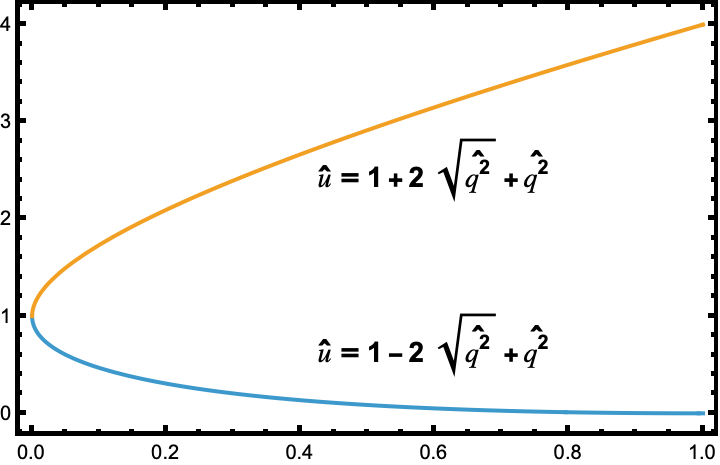
\includegraphics[width=\linewidth]{figures/singR1.png}
        \caption{实发射部分奇点分析1}
        \label{fig:sing_R1}
    \end{minipage}\hfill
    \begin{minipage}{0.5\textwidth}
        \centering
        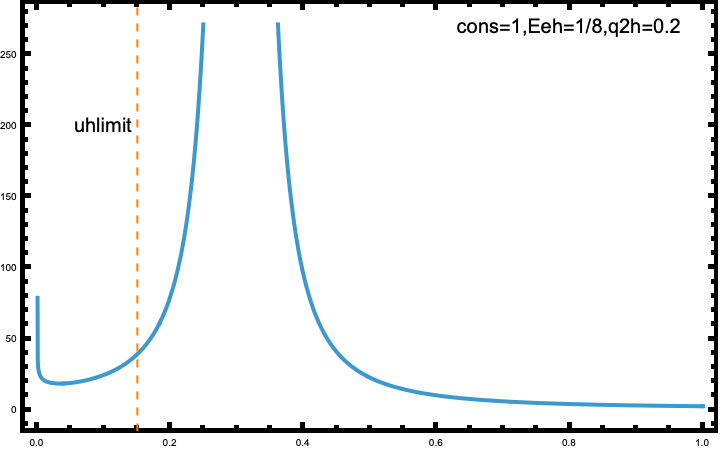
\includegraphics[width=\linewidth]{figures/singR2.png}
        \caption{实发射部分奇点分析2}
        \label{fig:sing_R2}
    \end{minipage}
\end{figure}
由于$\hat{u}$的物理区域是$\left[0,1\right]$，因此橙色曲线对应的奇点分布是非物理的。至于蓝色曲线对应的奇点分布，如图\ref{fig:sing_R2}所示，其中橙色虚线表示$\hat{u}$的积分上限，图中的发散区域对应于图\ref{fig:sing_R1}上$\hat{q^{2}}=0.25$附近，结果表明物理的奇点不在$\hat{u}$的积分区域以内。因此，式\eqref{eq:r_example}在$\hat{u}$的积分区域内不存在关于$\hat{u}$的不可积奇点。
\paragraph{B函数的相关项} 将三部分中的$B(\hat{u},{\hat{q^{2}}})$相关的项放在一起进行积分，其中最「奇异」的部分为：
    \begin{equation}
        \frac{2\left(2 \hat{E}_{\mathrm{e}}-\hat{q}^2-1\right)}{\hat{u}}\left[\left(2 \hat{E}_{\mathrm{e}}-\hat{q}^2\right) \mathcal{L}_2-\frac{\left(\hat{q}^2-1\right)\left(\hat{q}^2-2 \hat{E}_{\mathrm{e}}\right) \mathcal{L}_1}{\Delta}\right]
        \label{eq:B_example}
    \end{equation}
其中，$\Delta=\sqrt{\left(-\hat{q}^2+\hat{u}+1\right)^2-4 \hat{u}}$,$\mathcal{L}_1=\log \left(\frac{\Delta-\hat{q}^2+\hat{u}+1}{-\Delta-\hat{q}^2+\hat{u}+1}\right)$,$\mathcal{L}_2=\log \left(\frac{\hat{u}}{\left(\hat{q}^2-1\right)^2}\right)$。 式\eqref{eq:B_example}中似乎表明被积函数在$\hat{u}=0$处发散，对被积函数在$\hat{u}=0$处进行泰勒展开\footnote{泰勒展开的领头阶事实上对应于$\hat{u}$趋于零的极限}并分析发散行为\footnote{确定正规化参数取极限的方向以及积分限的偏移方向是必要的，否则会引入新的发散或错误，特别地，需要谨慎积分变量换元之后积分限的偏移方向。}是必要的。基于量子场论正规化思想，引入正规化常数$\epsilon$至积分区域边界处：
\begin{equation}
    \int_{0}^{1} f(\hat{u}) \mrm{d}\hat{u}\rightarrow\int_{\epsilon}^{1} f(\hat{u}) \mrm{d}\hat{u}\quad\quad \mrm{Im}(\epsilon)=0\text{且}\epsilon>0.
\end{equation}
积分完成后，取正规化参数趋于零的极限，结果表明式\eqref{eq:B_example}存在一个有限的积分结果。
\subsection{单圈水平上$\mrm{D\to X e^{+}\nu}$过程的领先幂次修正}
结合粲强子半轻单举衰变与底强子半轻单举衰变的区别，可得粲强子半轻单举衰变的电子能谱中对应于单圈水平上领先幂次修正的部分，电子能谱在电子能量的端点区域具有对数发散(可积发散)。对其进行加权积分，可得各类物理观测量的解析形式。

事实上，$\mrm{D\to X e^{+}\nu}$主要包含两个过程，分别是$\mrm{D\to X_s e^{+}}$和$\mrm{D\to X_d e^{+}\nu}$。对于前者，由于奇异夸克质量并非特别小，这里作为一个软自由度进行保留，有关末态有限夸克质量效应的修正，本文采用了Mannel等人\ct{Fael:2019umf}的工作。$\mrm{D\to X e^{+}\nu}$的衰变宽度为：
对于衰变宽度，
\begin{equation}
\begin{aligned}
    \Gamma_{D_{i}} = \sum_{q = \mathrm{d}, \mathrm{s}} \hat{\Gamma}_0 \mrm{\left| V_{\mathrm{c}q} \right|^2} m_{\mathrm{c}}^5 \Big\{ 1 & + \frac{\alpha_s}{\pi} \frac{2}{3} \left( \frac{25}{4} - \pi^2 \right)\\
    & + \frac{\alpha_s^2}{\pi^2} \left[ \frac{\beta_0}{4} \frac{2}{3} \left( \frac{25}{4} - \pi^2 \right) \log \left( \frac{\mu^2}{m_{\mathrm{c}}^2} \right) + 2.14690 n_l - 29.88311 \right]\\  
    &- 8 \rho \delta_{\mathrm{s}q} - \frac{1}{2} \frac{\mu_{\pi}^{2}(D_{i})}{m_{\mathrm{c}}^2} - \frac{3}{2} \frac{\mu_{\mathrm{G}}^{2}(D_{i})}{m_{\mathrm{c}}^2} + 6 \frac{\rho_{\mathrm{D}}^3\left(D_{i}\right)}{m_{\mathrm{c}}^3} + \dots \Big\},
\end{aligned}
\label{eq:decaywidth}
\end{equation}
式\eqref{eq:decaywidth}中，$\hat{\Gamma}_0 = {G_F^2 }/{(192 \pi^3)}$, $V_{cq}$ 是对应过程的CKM矩阵元，指标$i=u, d, s$分别指$\mrm{D^{+}}$,$\mrm{D^{0}}$和$\mrm{D_s^+}$, $\beta_0 = 11-2n_f /3$是量子色动力学$\beta$函数的第一个系数, $\rho\equiv m_s^2/m_c^2$. 对于微扰修正，$n_{f}=4$对应于$n_{l}=3$。本文微扰部分的单圈修正结果与DeFazio，Capdevila等人的工作一致\cite{DeFazio:1999ptt,Capdevila:2021vkf}. VanRitbergen和Brucherseifer等人讨论了$\mrm{b\to u}$过程的两圈图水平上领先幂次的修正，在衰变宽度的意义上，底强子弱衰变弱衰变$n_{f}=5$而粲强子单举弱衰变的$n_{f}=4$。本文关于两圈图修正的数值结果由陈龙、马滟青老师提供。
关于\ref{eq:decaywidth}中非微扰矩阵元的定义，本文采用Mannel等人的约定\ct{Fael:2019umf}：
\begin{equation}
    \begin{aligned}
        \mu_\pi^2(D_i) &\equiv \langle D_i| \bar c_v(iD)^2 c_v| D_i \rangle /(2m_{D_i}) , \; \\
        \mu_G^2(D_i) &\equiv \langle D_i| \bar c_v (iD_\alpha)(iD_\beta)(-i\sigma^{\alpha\beta}) c_v| D_i \rangle  /(2m_{D_i}),  \\
        \rho_{LS}^3(D_i) &\equiv {1\over2}\langle D_i| \bar c_v \{(iD_\alpha), [iv\cdot D, iD_\beta ]\} (-i\sigma^{\alpha\beta})| D_i \rangle /(2m_{D_i}) , \;\\ 
        \rho^3_{D}(D_i) &\equiv {1\over2}\langle D_i| \bar c_v  [(iD^\mu), [iv\cdot D, iD_\mu]] c_v | D_i \rangle /(2m_{D_i}). \; \\
        \end{aligned}
\end{equation}
      n阶电子能量原点矩，其定义如下
      \begin{equation}
        \langle E_{\mathrm{e}}^{n} \rangle = \frac{1}{\Gamma} \int \hat{E}_{\mathrm{e}}^{n} \frac{d \Gamma}{d \hat{E}_{\mathrm{e}}} \, d \hat{E}_{\mathrm{e}},
\end{equation}
      其中， $\Gamma$是衰变宽度，$n=1, 2, 3\cdots$.
      对电子能谱进行加权积分，前四阶电子能量（原点）矩.
      如下所示，
      \begin{equation}
        \scriptsize
        \begin{aligned}
            \langle E_{e}\rangle_{D_{i}}&=\frac{\hat{\Gamma}_0}{    \Gamma_{D_{i}}}\sum_{q=d,s} \left|V_{cq}\right|^2 m_{c}^6 \left[\frac{3}{10} + \frac{\alpha_{s}}{\pi} a_1^{(1)} + {\alpha_s^2\over \pi^2}a_1^{(2)} -3\rho\delta_{sq} -\frac{1}{2}\frac{\mu_{G}^{2}(D_{i})}{m_{c}^{2}} +\frac{139}{30} \frac{\rho_D^3\left(D_{i}\right)}{m_c^3}+\frac{3}{10} \frac{\rho_{L S}^3\left(D_{i}\right)}{m_c^3}+ ...\right],\\
            \langle E_{e}^{2} \rangle_{D_{i}} &=\frac{\hat{\Gamma}_0}{\Gamma_{D_{i}}} \sum_{q=d,s}\left|V_{cq}\right|^2 m_c^7 \left[ \frac{1}{10} + \frac{\alpha_{s}}{\pi} a_2^{(1)}  + {\alpha_s^2\over \pi^2}a_2^{(2)}  - \frac{6}{5} \rho\delta_{sq} + \frac{1}{12}\frac{\mu_{\pi}^2(D_{i})}{ m_c^2} - \frac{11}{60}\frac{\mu_G^2(D_{i})}{ m_c^2} +\frac{17}{6} \frac{\rho_D^3\left(D_{i}\right)}{m_c^3} \right.\nonumber \\
            &\qquad\qquad\qquad\qquad\qquad \left. +\frac{7}{30} \frac{\rho_{L S}^3\left(D_{i}\right)}{m_c^3}+ ... \right], \nonumber\\
            \left\langle E_e^3\right\rangle_{D_{i}}&=\frac{\hat{\Gamma}_0}{\Gamma_{D_{i}}}\sum_{q=d,s}\left|V_{cq}\right|^2 m_c^8\left[\frac{1}{28} + \frac{\alpha_{s}}{\pi} a_3^{(1)}  + {\alpha_s^2\over \pi^2}a_3^{(2)}  -\frac{1}{2} \rho\delta_{sq} +\frac{1}{14} \frac{\mu_\pi^2\left(D_{i}\right)}{ m_c^2}-\frac{1}{14} \frac{\mu_G^2\left(D_{i}\right)}{ m_c^2}+\frac{223}{140} \frac{\rho_D^3\left(D_{i}\right)}{m_c^3}\right. \nonumber\\
            &\qquad\qquad\qquad\qquad\qquad \left.+\frac{1}{7} \frac{\rho_{L S}^3\left(D_{i}\right)}{m_c^3} + ... \right],\nonumber\\
            \left\langle E_e^4\right\rangle_{D_i}&=\frac{\hat{\Gamma}_0}{\Gamma_{D_{i}}}\sum_{q=d,s}\left|V_{cq}\right|^2 m_c^9\left[\frac{3}{224} + \frac{\alpha_{s}}{\pi} a_4^{(1)}  + {\alpha_s^2\over \pi^2}a_4^{(2)}  -\frac{3}{14} \rho\delta_{sq} +\frac{3}{64} \frac{\mu_\pi^2\left(D_{i}\right)}{ m_c^2}-\frac{13}{448} \frac{\mu_G^2\left(D_{i}\right)}{ m_c^2} +\frac{481}{560} \frac{\rho_D^3\left(D_i\right)}{m_c^3}\right. \nonumber\\
            &\qquad\qquad\qquad\qquad\qquad \left.+\frac{9}{112} \frac{\rho_{L S}^3\left(D_i\right)}{m_c^3}+ ... \right],\nonumber
            \end{aligned}
            \label{eq:inital_moments}
      \end{equation}
      式\eqref{eq:inital_moments}的NLO和NNLO系数如下所示，
      \begin{equation}
        \scriptsize
      \begin{aligned}
        a^{(1)}_1 &= {1093 - 180\pi^2\over 900 }, \;
        a^{(1)}_2 = \frac{4243 - 720 \pi^2}{{10800}}, \; 
        a^{(1)}_3 = \frac{144037-25200 \pi^2}{{1058400}}, \; 
        a^{(1)}_4 = \frac{69827-12600 \pi^2}{{1411200}},   \\
        a^{(2)}_1 &= {\beta_0\over 4}a^{(1)}_1\ell -7.70077, \; 
        a^{(2)}_2 = {\beta_0\over 4}a^{(1)}_2\ell -2.77835, \; 
        a^{(2)}_3 = {\beta_0\over 4}a^{(1)}_3\ell -1.06371 , \; 
        a^{(2)}_4 = {\beta_0\over 4}a^{(1)}_4\ell -0.42438 , \nonumber
        \end{aligned}
    \end{equation}
        本文关于前两阶电子能量（原点）矩的结果与Kamenik等人的工作\cite{Kamenik:2011zz}一致，树图水平上量纲六算符的修正来源于Mannel等人的工作\cite{Fael:2019umf}，前四阶矩的领头阶与Mannel等人的结果\cite{Fael:2019umf}一致。
        事实上，本文同样提供了电子能量第二、三、四阶的中心矩，电子能量的中心矩由原点矩线性组合而成，定义如下：
        \begin{equation}
            \scriptsize
        \begin{aligned}
            \left\langle E_e\right\rangle, \;\left\langle E_e^2\right\rangle_{\rm center}\equiv \left\langle (E_e - \langle E_e\rangle)^2 \right\rangle , \; \left\langle E_e^3\right\rangle_{\rm center}\equiv\left\langle (E_e - \langle E_e\rangle)^3 \right\rangle , \; \left\langle E_e^4\right\rangle_{\rm center}\equiv\left\langle (E_e - \langle E_e\rangle)^4 \right\rangle .
            \end{aligned}
        \end{equation}
    由于物理可观测量对粲夸克质量的高度敏感性，有关粲夸克质量方案的讨论是必要的，具体讨论将在第四章全局拟合的部分呈现。
\section{更高量纲算符非微扰矩阵元的参数化}
上一节通过对电子能谱的加权积分得到各类物理可观测量，其中量纲六算符非微扰矩阵元的贡献来自于Mannel等人的工作\ct{Fael:2019umf}。本节基于Lenz等人的工作\ct{King:2021jsq}对量纲六算符非微扰矩阵元的参数化进行简单介绍。

量纲六算符分为两夸克算符和四夸克算符，对于两夸克算符，仅$\rho_{D}^{3}$对衰变宽度由贡献，其非微扰矩阵元可做如下的参数化
\begin{equation}
    2 m_D \rho_D^3(D)=\langle D(p)| \bar{c}_v\left(i D_\mu\right)(i v \cdot D)\left(i D^\mu\right) c_v|D(p)\rangle .
    \end{equation}
    在衰变宽度的水平上，
    \begin{equation}
        \Gamma_6 \frac{\left\langle\mathcal{O}_6\right\rangle}{m_c^3}=\Gamma_0 c_{\rho_D} \frac{\rho_D^3}{m_c^3}
        \end{equation}
    其中,$\Gamma_{0}=\frac{G_F^2 m_c^5 V_{\text{CKM}}}{192\pi^3}$, $c_{\rho_D}=3 C_1^2 \mathcal{C}_{\rho_D, 11}+2 C_1 C_2 \mathcal{C}_{\rho_D, 12}+3 C_2^2 \mathcal{C}_{\rho_D, 22}+\mathcal{C}_{\rho_D, \mrm{S L}}$.

    对于底强子弱衰变过程，Lenz，Mannel和Daniel等人的工作\ct{Lenz:2020oce,Mannel:2020fts,Moreno:2020rmk}给出了非轻部分的Wilson系数，其中需要处理来自轻自由度的软胶子辐射，会导致$\ln(m_{q}/m_{b})$的对数发散，事实上，将四夸克算符以及算符混合的贡献考虑在内，则可以完全消除； 对于底强子的半轻衰变，由于$\rho=m_\mrm{c}^2/m_\mrm{b}^2$不是一个小量，$\mrm{b\to c e\nu_e}$过程量纲六算符的Wilson系数是有限的，但中间无质量传播子发射软胶子使得$b\to u e\nu $过程量纲六算符对应的Wilson系数存在发散。
    
    对于粲强子弱衰变过程，由于，$m_{\mrm{c}}>>m_{s}\sim \Lambda_{QCD}$，因此末态奇异夸克质量作为软自由度与四夸克算符的混合需要额外考虑， Lenz等人的工作\ct{King:2021xqp}讨论了这部分的Wilson系数，并将其用于D介子寿命的理论计算。
    
    量纲六算符中四夸克算符来源于旁观者夸克效应，存在以下三种贡献(图\ref{fig:spector})，
    \begin{figure}[h!]
        \centering
        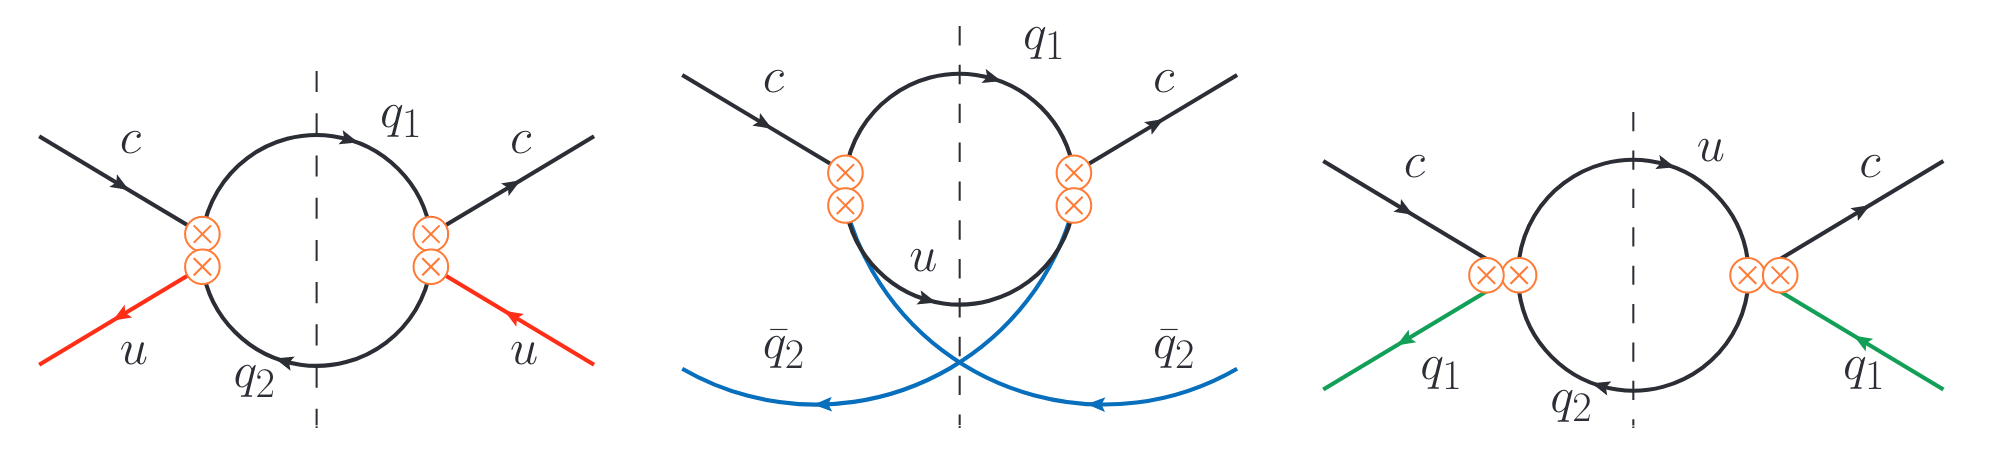
\includegraphics[width=\textwidth]{figures/spector.png}
        \caption{重夸克展开的旁观者夸克效应拓扑图\ct{King:2021xqp}}
        \label{fig:spector}
    \end{figure}
图\ref{fig:spector}中从左至右分别是弱交换（Weak Exchange， WE）、泡利干涉（Pauli Interference，PI）和弱湮灭（Weak Annihilation，WA）贡献\footnote{半轻衰变只存在弱湮灭贡献}。量纲六算符中的四夸克算符如下所示\footnote{两个等号表示存在两种记号}
\begin{equation}
    \begin{aligned}
    & O_1^q=\left(\bar{c} \gamma_\mu\left(1-\gamma_5\right) q\right)\left(\bar{q} \gamma^\mu\left(1-\gamma_5\right) c\right), \\
    & O_2^q=\left(\bar{c}\left(1-\gamma_5\right) q\right)\left(\bar{q}\left(1+\gamma_5\right) c\right), \\
    & O_3^q=T_1^q=\left(\bar{c} \gamma_\mu\left(1-\gamma_5\right) T^A q\right)\left(\bar{q} \gamma^\mu\left(1-\gamma_5\right) T^A c\right), \\
    & O_4^q=T_2^q=\left(\bar{c}\left(1-\gamma_5\right) T^A q\right)\left(\bar{q}\left(1+\gamma_5\right) T^A c\right),
    \end{aligned}
    \end{equation}
在量子色动力学框架下，其非微扰矩阵元进行如下的参数化，
\begin{equation}
    \begin{aligned}
    \left\langle D_q\right| O_i^q\left|D_q\right\rangle & =A_i f_{D_q}^2 m_{D_q}^2 B_i^q \\
    \left\langle D_q\right| O_i^{q^{\prime}}\left|D_q\right\rangle & =A_i f_{D_q}^2 m_{D_q}^2 \delta_i^{q q^{\prime}}, \quad q \neq q^{\prime}
    \end{aligned}
    \end{equation}
    其中，$A_1^q=A_3^q=1, \quad A_2^q=A_4^q=\frac{m_D^2}{\left(m_c+m_q\right)^2}$，$f^2_{D_{q}}$量子色动力学框架下的$D_{q}$介子的衰变常数，$m_{D_{q}}$是$D_{q}$质量，$B_{i}^{q}$是Bag 参数。
在重夸克有效理论框架下，量纲六算符中的四夸克算符为：
\begin{equation}
    \begin{aligned}
    & \tilde{O}_1^q=\left(\bar{h}_v \gamma_\mu\left(1-\gamma_5\right) q\right)\left(\bar{q} \gamma^\mu\left(1-\gamma_5\right) h_v\right), \\
    & \tilde{O}_2^q=\left(\bar{h}_v\left(1-\gamma_5\right) q\right)\left(\bar{q}\left(1+\gamma_5\right) h_v\right), \\
    & \tilde{O}_3^q=\tilde{T}_1^q=\left(\bar{h}_v \gamma_\mu\left(1-\gamma_5\right) T^A q\right)\left(\bar{q} \gamma^\mu\left(1-\gamma_5\right) T^A h_v\right), \\
    & \tilde{O}_4^q=\tilde{T}_2^q=\left(\bar{h}_v\left(1-\gamma_5\right) T^A q\right)\left(\bar{q}\left(1+\gamma_5\right) T^A h_v\right),
    \end{aligned}
    \end{equation}
其中$h_{v}$是积掉重自由度的有效重夸克场，量纲六算符中的四夸克算符可以进行如下的参数化，
\begin{equation}
    \begin{aligned}
    \left\langle D_q\right| \tilde{O}_i^q\left|D_q\right\rangle & =F^2(\mu) m_{D_q} \tilde{B}_i^q \\
    \left\langle D_q\right| \tilde{O}_i^{q^{\prime}}\left|D_q\right\rangle & =F^2(\mu) m_{D_q} \tilde{\delta}_i^{q^{\prime} q}, \quad q \neq q^{\prime},
    \end{aligned}
    \label{eq:dim6_4_parameters}
    \end{equation}
    其中$q, q^{\prime}=u, d, s, \tilde{B}_i^q$表示HQET中的Bag参数，$\tilde{B}_{1,2}^q$对应于色单态算符，$\tilde{B}_{3,4}^q \equiv \tilde{\epsilon}_{1,2}^q$对应于色八态算符，$F(\mu)$是HQET衰变常数。
    \begin{equation}
        \begin{aligned}
            \langle 0| \bar{q} \gamma^\mu \gamma_5 h_v\left|D_q(v)\right\rangle_{\mathrm{HQET}}&=i F(\mu) \sqrt{m_{D_q}} v^\mu,\\
            \langle 0| \bar{q} \gamma^\mu \gamma_5 c\left|D_q(p)\right\rangle_{\mathrm{QCD}}&=i f_{D_q} p^\mu
        \end{aligned}
        \end{equation}
    \paragraph{真空插入近似假设(vacuum insertion approximation, VIA)}为简化强子内部相互作用，近似假设强子内为真空态，其色场被近似为色单态。具体地，在四夸克算符矩阵元中插入一组完备集，仅保留真空态贡献，将四夸克算符非微扰矩阵元因子化为衰变常数和Bag参数的乘积，Bag参数依赖于算符中的色结构。
    色单态算符对应的Bag参数为假设为1， 色八重态算符对应的Bag参数被假设为0。

    式\eqref{eq:dim6_4_parameters}中的$\tilde{\delta}_i^{q^{\prime} q}$描述了eye-contractions,如图\ref{fig:eye}所示，eye-contractions指由于内外夸克之间的相互作用，它们以一种特定的方式被连接起来。
    \begin{figure}[h!]
        \centering
        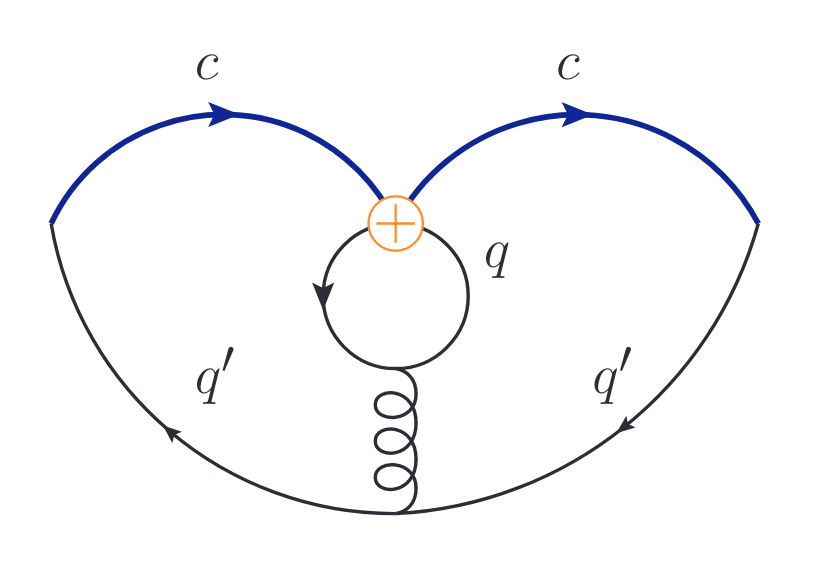
\includegraphics[width=0.4\textwidth]{figures/eye.png}
        \caption{量纲六算符非微扰矩阵元之一：Eye-contractions 效应\ct{King:2021xqp}}
        \label{fig:eye}
    \end{figure}
     
    受到$\alpha_s$的压低，真空插入近似下，Eye-contractions贡献被假设为零。在重夸克有效理论求和规则中（Heavy Quark Effective Theory Sum Rule, HQETSR），表征Eye-contractions的参数$\tilde{\delta}_i^{q^{\prime} q}$则并不严格为零。
    \begin{table}[h!]
        \centering
        \small % 或 \footnotesize 进一步缩小
        \setlength{\tabcolsep}{4pt} % 减少列间距
        \renewcommand{\arraystretch}{1.1} % 微调行高
        \begin{tabular}{|c||c|c|c|c|}
            \hline 
            HQET, $\mu_0=1.5 \mathrm{GeV}$ & $\tilde{B}_1$ & $\tilde{B}_2$ & $\tilde{\epsilon}_1$ & $\tilde{\epsilon}_2$ \\
            \hline
            $D^{+, 0}$ & $1.0026_{-0.0106}^{+0.0198}$ & $0.9982_{-0.0066}^{+0.0052}$ & $-0.0165_{-0.0346}^{+0.0209}$ & $-0.0004_{-0.0326}^{+0.0200}$ \\
            \hline
            $D_s^{+}$ & $1.0022_{-0.0099}^{+0.0185}$ & $0.9983_{-0.0067}^{+0.0052}$ & $-0.0104_{-0.0330}^{+0.0202}$ & $0.0001_{-0.0324}^{+0.0199}$ \\
            \hline \hline 
            HQET, $\mu_0=1.5 \mathrm{GeV}$ & $\tilde{\delta}_1$ & $\tilde{\delta}_2$ & $\tilde{\delta}_3$ & $\tilde{\delta}_4$ \\
            \hline
            $\left\langle D_q\right| \tilde{O}^q\left|D_q\right\rangle$ & $0.0026_{-0.0092}^{+0.0142}$ & $-0.0018_{-0.0072}^{+0.0047}$ & $-0.0004_{-0.0024}^{+0.0015}$ & $0.0003_{-0.0008}^{+0.0012}$ \\
            \hline
            $\left\langle D_s\right| \tilde{O}^q\left|D_s\right\rangle$ & $0.0025_{-0.0093}^{+0.014}$ & $-0.0018_{-0.0072}^{+0.0047}$ & $-0.0004_{-0.0024}^{+0.0015}$ & $0.0003_{-0.0008}^{+0.0012}$ \\
            \hline
            $\left\langle D_q\right| \tilde{O}^s\left|D_q\right\rangle$ & $0.0023_{-0.0091}^{+0.0140}$ & $-0.0017_{-0.0070}^{+0.0046}$ & $-0.0004_{-0.0023}^{+0.0015}$ & $0.0003_{-0.0008}^{+0.0012}$ \\
            \hline
        \end{tabular}
        \caption{HQETSR关于Bag参数的数值结果}
        \label{tab:HQETSR_num_Bag}
    \end{table}
    值得注意的是，\(\mrm{ D^{+, 0}} \) 介子的 Bag 参数 \( \tilde{B}_i^q \) 的HQETSR的预言由Lenz等人的工作\ct{Kirk:2017juj}给出,同时他们也给出了Eye-contractions效应的HQETSR的预言\ct{King:2021jsq}。如表\ref{tab:HQETSR_num_Bag}所示，
基于真空插入近似，表征Eye-contractions效应的参数和色八重态算符对应的Bag参数被假设为零，色单态算符非微扰矩阵元收到相应Wilson系数压低，这是我们从实验数据中抽取量纲五算符和量纲六算符两夸克算符非微扰矩阵元的理论依据。
\section{本章回顾}
基于第二章关于重夸克有效理论和算符乘积简单介绍，深入介绍了本文理论方面的努力。首先基于Mark.B.Wise的经典教材\ct{manohar2000heavy}介绍了$\mrm{\mrm{B}\to X_{c}e\nu}$过程Wilson系数的匹配和末态相空间的解析积分,获得该过程以及$\mrm{\mrm{B}\to X_{u}e\nu}$过程电子能谱的解析形式；其次，基于更现代的运动学变量对$\mrm{\mrm{B}\to X_{c}e\nu}$过程进行相同的讨论，并给出两组运动学变量（运动学参数化方案）之间的联系；此外，基于更现代的运动学变量对$\mrm{\mrm{B}\to X_{c}e\nu}$过程领先幂次修正的单圈微扰修正进行讨论，并推广至$\mrm{\mrm{B}\to X_{u}e\nu}$过程；最后，本章将有关B介子半轻单举衰变的讨论转换到$\mrm{D\to X e^{+}\nu}$过程，对电子能谱进行加权积分，获得了衰变宽度、电子能量一、二、三、四阶原点矩。以上的讨论为D介子半轻单举衰变的系统性唯象学分析奠定了理论基础。